\begin{figure}[H] \centering % Created by tikzDevice version 0.12.4 on 2023-08-13 18:28:52
% !TEX encoding = UTF-8 Unicode
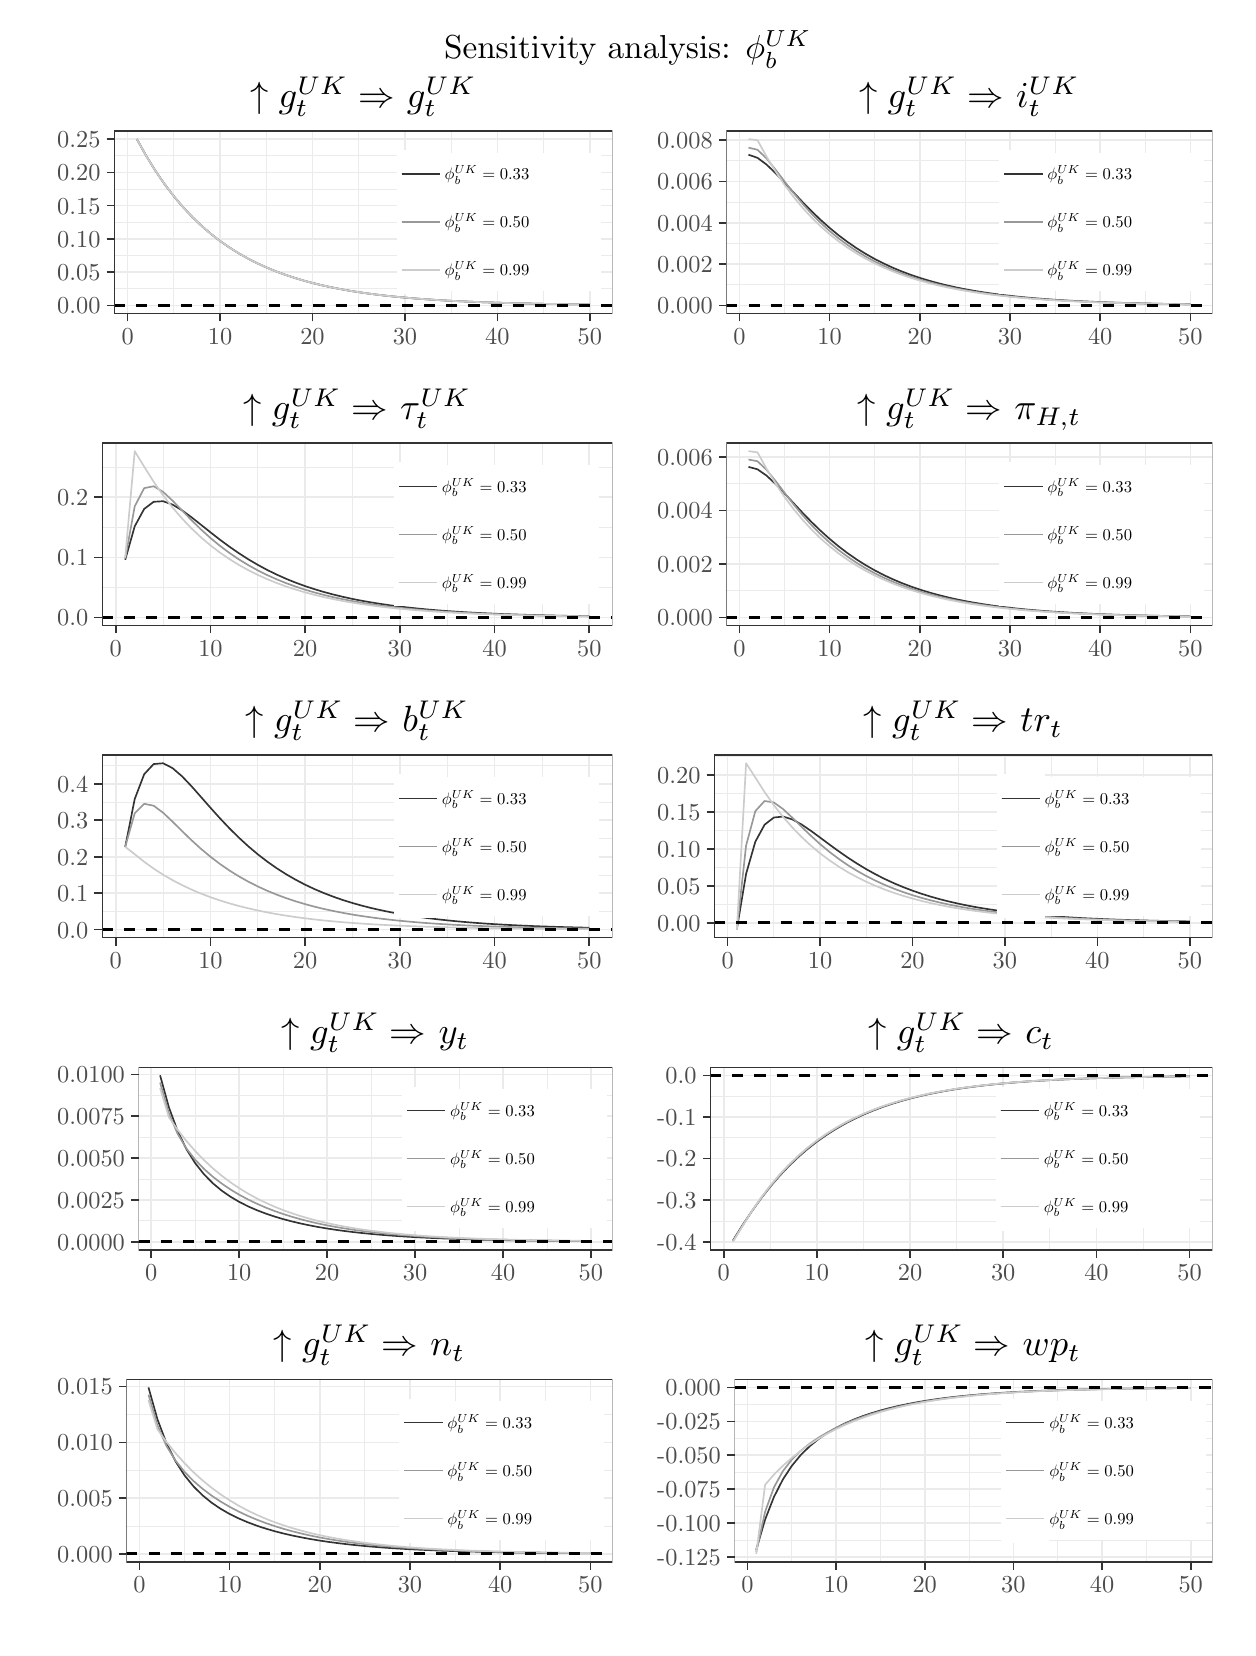
\begin{tikzpicture}[x=1pt,y=1pt]
\definecolor{fillColor}{RGB}{255,255,255}
\path[use as bounding box,fill=fillColor,fill opacity=0.00] (0,0) rectangle (433.62,578.16);
\begin{scope}
\path[clip] (  0.00,451.10) rectangle (216.81,563.87);
\definecolor{drawColor}{RGB}{255,255,255}
\definecolor{fillColor}{RGB}{255,255,255}

\path[draw=drawColor,line width= 0.6pt,line join=round,line cap=round,fill=fillColor] (  0.00,451.10) rectangle (216.81,563.87);
\end{scope}
\begin{scope}
\path[clip] ( 31.27,474.78) rectangle (211.31,540.91);
\definecolor{fillColor}{RGB}{255,255,255}

\path[fill=fillColor] ( 31.27,474.78) rectangle (211.31,540.91);
\definecolor{drawColor}{gray}{0.92}

\path[draw=drawColor,line width= 0.3pt,line join=round] ( 31.27,483.79) --
	(211.31,483.79);

\path[draw=drawColor,line width= 0.3pt,line join=round] ( 31.27,495.82) --
	(211.31,495.82);

\path[draw=drawColor,line width= 0.3pt,line join=round] ( 31.27,507.84) --
	(211.31,507.84);

\path[draw=drawColor,line width= 0.3pt,line join=round] ( 31.27,519.87) --
	(211.31,519.87);

\path[draw=drawColor,line width= 0.3pt,line join=round] ( 31.27,531.89) --
	(211.31,531.89);

\path[draw=drawColor,line width= 0.3pt,line join=round] ( 52.81,474.78) --
	( 52.81,540.91);

\path[draw=drawColor,line width= 0.3pt,line join=round] ( 86.22,474.78) --
	( 86.22,540.91);

\path[draw=drawColor,line width= 0.3pt,line join=round] (119.62,474.78) --
	(119.62,540.91);

\path[draw=drawColor,line width= 0.3pt,line join=round] (153.02,474.78) --
	(153.02,540.91);

\path[draw=drawColor,line width= 0.3pt,line join=round] (186.43,474.78) --
	(186.43,540.91);

\path[draw=drawColor,line width= 0.6pt,line join=round] ( 31.27,477.78) --
	(211.31,477.78);

\path[draw=drawColor,line width= 0.6pt,line join=round] ( 31.27,489.81) --
	(211.31,489.81);

\path[draw=drawColor,line width= 0.6pt,line join=round] ( 31.27,501.83) --
	(211.31,501.83);

\path[draw=drawColor,line width= 0.6pt,line join=round] ( 31.27,513.86) --
	(211.31,513.86);

\path[draw=drawColor,line width= 0.6pt,line join=round] ( 31.27,525.88) --
	(211.31,525.88);

\path[draw=drawColor,line width= 0.6pt,line join=round] ( 31.27,537.90) --
	(211.31,537.90);

\path[draw=drawColor,line width= 0.6pt,line join=round] ( 36.11,474.78) --
	( 36.11,540.91);

\path[draw=drawColor,line width= 0.6pt,line join=round] ( 69.52,474.78) --
	( 69.52,540.91);

\path[draw=drawColor,line width= 0.6pt,line join=round] (102.92,474.78) --
	(102.92,540.91);

\path[draw=drawColor,line width= 0.6pt,line join=round] (136.32,474.78) --
	(136.32,540.91);

\path[draw=drawColor,line width= 0.6pt,line join=round] (169.72,474.78) --
	(169.72,540.91);

\path[draw=drawColor,line width= 0.6pt,line join=round] (203.13,474.78) --
	(203.13,540.91);
\definecolor{drawColor}{gray}{0.20}

\path[draw=drawColor,line width= 0.6pt,line join=round] ( 39.45,537.90) --
	( 42.79,531.89) --
	( 46.13,526.48) --
	( 49.47,521.61) --
	( 52.81,517.23) --
	( 56.15,513.28) --
	( 59.50,509.73) --
	( 62.84,506.54) --
	( 66.18,503.66) --
	( 69.52,501.07) --
	( 72.86,498.75) --
	( 76.20,496.65) --
	( 79.54,494.76) --
	( 82.88,493.06) --
	( 86.22,491.54) --
	( 89.56,490.16) --
	( 92.90,488.92) --
	( 96.24,487.81) --
	( 99.58,486.81) --
	(102.92,485.90) --
	(106.26,485.09) --
	(109.60,484.36) --
	(112.94,483.70) --
	(116.28,483.11) --
	(119.62,482.58) --
	(122.96,482.10) --
	(126.30,481.67) --
	(129.64,481.28) --
	(132.98,480.93) --
	(136.32,480.61) --
	(139.66,480.33) --
	(143.00,480.08) --
	(146.34,479.85) --
	(149.68,479.64) --
	(153.02,479.45) --
	(156.36,479.29) --
	(159.70,479.14) --
	(163.04,479.00) --
	(166.38,478.88) --
	(169.72,478.77) --
	(173.06,478.67) --
	(176.40,478.58) --
	(179.74,478.50) --
	(183.08,478.43) --
	(186.43,478.36) --
	(189.77,478.31) --
	(193.11,478.25) --
	(196.45,478.21) --
	(199.79,478.16) --
	(203.13,478.13);
\definecolor{drawColor}{RGB}{152,152,152}

\path[draw=drawColor,line width= 0.6pt,line join=round] ( 39.45,537.90) --
	( 42.79,531.89) --
	( 46.13,526.48) --
	( 49.47,521.61) --
	( 52.81,517.23) --
	( 56.15,513.28) --
	( 59.50,509.73) --
	( 62.84,506.54) --
	( 66.18,503.66) --
	( 69.52,501.07) --
	( 72.86,498.75) --
	( 76.20,496.65) --
	( 79.54,494.76) --
	( 82.88,493.06) --
	( 86.22,491.54) --
	( 89.56,490.16) --
	( 92.90,488.92) --
	( 96.24,487.81) --
	( 99.58,486.81) --
	(102.92,485.90) --
	(106.26,485.09) --
	(109.60,484.36) --
	(112.94,483.70) --
	(116.28,483.11) --
	(119.62,482.58) --
	(122.96,482.10) --
	(126.30,481.67) --
	(129.64,481.28) --
	(132.98,480.93) --
	(136.32,480.61) --
	(139.66,480.33) --
	(143.00,480.08) --
	(146.34,479.85) --
	(149.68,479.64) --
	(153.02,479.45) --
	(156.36,479.29) --
	(159.70,479.14) --
	(163.04,479.00) --
	(166.38,478.88) --
	(169.72,478.77) --
	(173.06,478.67) --
	(176.40,478.58) --
	(179.74,478.50) --
	(183.08,478.43) --
	(186.43,478.36) --
	(189.77,478.31) --
	(193.11,478.25) --
	(196.45,478.21) --
	(199.79,478.16) --
	(203.13,478.13);
\definecolor{drawColor}{gray}{0.80}

\path[draw=drawColor,line width= 0.6pt,line join=round] ( 39.45,537.90) --
	( 42.79,531.89) --
	( 46.13,526.48) --
	( 49.47,521.61) --
	( 52.81,517.23) --
	( 56.15,513.28) --
	( 59.50,509.73) --
	( 62.84,506.54) --
	( 66.18,503.66) --
	( 69.52,501.07) --
	( 72.86,498.75) --
	( 76.20,496.65) --
	( 79.54,494.76) --
	( 82.88,493.06) --
	( 86.22,491.54) --
	( 89.56,490.16) --
	( 92.90,488.92) --
	( 96.24,487.81) --
	( 99.58,486.81) --
	(102.92,485.90) --
	(106.26,485.09) --
	(109.60,484.36) --
	(112.94,483.70) --
	(116.28,483.11) --
	(119.62,482.58) --
	(122.96,482.10) --
	(126.30,481.67) --
	(129.64,481.28) --
	(132.98,480.93) --
	(136.32,480.61) --
	(139.66,480.33) --
	(143.00,480.08) --
	(146.34,479.85) --
	(149.68,479.64) --
	(153.02,479.45) --
	(156.36,479.29) --
	(159.70,479.14) --
	(163.04,479.00) --
	(166.38,478.88) --
	(169.72,478.77) --
	(173.06,478.67) --
	(176.40,478.58) --
	(179.74,478.50) --
	(183.08,478.43) --
	(186.43,478.36) --
	(189.77,478.31) --
	(193.11,478.25) --
	(196.45,478.21) --
	(199.79,478.16) --
	(203.13,478.13);
\definecolor{drawColor}{RGB}{0,0,0}

\path[draw=drawColor,line width= 1.1pt,dash pattern=on 4pt off 4pt ,line join=round] ( 31.27,477.78) -- (211.31,477.78);
\definecolor{drawColor}{gray}{0.20}

\path[draw=drawColor,line width= 0.6pt,line join=round,line cap=round] ( 31.27,474.78) rectangle (211.31,540.91);
\end{scope}
\begin{scope}
\path[clip] (  0.00,  0.00) rectangle (433.62,578.16);
\definecolor{drawColor}{gray}{0.30}

\node[text=drawColor,anchor=base east,inner sep=0pt, outer sep=0pt, scale=  0.88] at ( 26.32,474.75) {0.00};

\node[text=drawColor,anchor=base east,inner sep=0pt, outer sep=0pt, scale=  0.88] at ( 26.32,486.78) {0.05};

\node[text=drawColor,anchor=base east,inner sep=0pt, outer sep=0pt, scale=  0.88] at ( 26.32,498.80) {0.10};

\node[text=drawColor,anchor=base east,inner sep=0pt, outer sep=0pt, scale=  0.88] at ( 26.32,510.83) {0.15};

\node[text=drawColor,anchor=base east,inner sep=0pt, outer sep=0pt, scale=  0.88] at ( 26.32,522.85) {0.20};

\node[text=drawColor,anchor=base east,inner sep=0pt, outer sep=0pt, scale=  0.88] at ( 26.32,534.87) {0.25};
\end{scope}
\begin{scope}
\path[clip] (  0.00,  0.00) rectangle (433.62,578.16);
\definecolor{drawColor}{gray}{0.20}

\path[draw=drawColor,line width= 0.6pt,line join=round] ( 28.52,477.78) --
	( 31.27,477.78);

\path[draw=drawColor,line width= 0.6pt,line join=round] ( 28.52,489.81) --
	( 31.27,489.81);

\path[draw=drawColor,line width= 0.6pt,line join=round] ( 28.52,501.83) --
	( 31.27,501.83);

\path[draw=drawColor,line width= 0.6pt,line join=round] ( 28.52,513.86) --
	( 31.27,513.86);

\path[draw=drawColor,line width= 0.6pt,line join=round] ( 28.52,525.88) --
	( 31.27,525.88);

\path[draw=drawColor,line width= 0.6pt,line join=round] ( 28.52,537.90) --
	( 31.27,537.90);
\end{scope}
\begin{scope}
\path[clip] (  0.00,  0.00) rectangle (433.62,578.16);
\definecolor{drawColor}{gray}{0.20}

\path[draw=drawColor,line width= 0.6pt,line join=round] ( 36.11,472.03) --
	( 36.11,474.78);

\path[draw=drawColor,line width= 0.6pt,line join=round] ( 69.52,472.03) --
	( 69.52,474.78);

\path[draw=drawColor,line width= 0.6pt,line join=round] (102.92,472.03) --
	(102.92,474.78);

\path[draw=drawColor,line width= 0.6pt,line join=round] (136.32,472.03) --
	(136.32,474.78);

\path[draw=drawColor,line width= 0.6pt,line join=round] (169.72,472.03) --
	(169.72,474.78);

\path[draw=drawColor,line width= 0.6pt,line join=round] (203.13,472.03) --
	(203.13,474.78);
\end{scope}
\begin{scope}
\path[clip] (  0.00,  0.00) rectangle (433.62,578.16);
\definecolor{drawColor}{gray}{0.30}

\node[text=drawColor,anchor=base,inner sep=0pt, outer sep=0pt, scale=  0.88] at ( 36.11,463.76) {0};

\node[text=drawColor,anchor=base,inner sep=0pt, outer sep=0pt, scale=  0.88] at ( 69.52,463.76) {10};

\node[text=drawColor,anchor=base,inner sep=0pt, outer sep=0pt, scale=  0.88] at (102.92,463.76) {20};

\node[text=drawColor,anchor=base,inner sep=0pt, outer sep=0pt, scale=  0.88] at (136.32,463.76) {30};

\node[text=drawColor,anchor=base,inner sep=0pt, outer sep=0pt, scale=  0.88] at (169.72,463.76) {40};

\node[text=drawColor,anchor=base,inner sep=0pt, outer sep=0pt, scale=  0.88] at (203.13,463.76) {50};
\end{scope}
\begin{scope}
\path[clip] (  0.00,  0.00) rectangle (433.62,578.16);
\definecolor{fillColor}{RGB}{255,255,255}

\path[fill=fillColor] (134.34,482.83) rectangle (207.26,532.86);
\end{scope}
\begin{scope}
\path[clip] (  0.00,  0.00) rectangle (433.62,578.16);
\definecolor{fillColor}{RGB}{255,255,255}

\path[fill=fillColor] (133.34,516.52) rectangle (150.69,533.86);
\end{scope}
\begin{scope}
\path[clip] (  0.00,  0.00) rectangle (433.62,578.16);
\definecolor{drawColor}{gray}{0.20}

\path[draw=drawColor,line width= 0.6pt,line join=round] (135.08,525.19) -- (148.95,525.19);
\end{scope}
\begin{scope}
\path[clip] (  0.00,  0.00) rectangle (433.62,578.16);
\definecolor{drawColor}{gray}{0.20}

\path[draw=drawColor,line width= 0.6pt,line join=round] (135.08,525.19) -- (148.95,525.19);
\end{scope}
\begin{scope}
\path[clip] (  0.00,  0.00) rectangle (433.62,578.16);
\definecolor{drawColor}{gray}{0.20}

\path[draw=drawColor,line width= 0.6pt,line join=round] (135.08,525.19) -- (148.95,525.19);
\end{scope}
\begin{scope}
\path[clip] (  0.00,  0.00) rectangle (433.62,578.16);
\definecolor{fillColor}{RGB}{255,255,255}

\path[fill=fillColor] (133.34,499.17) rectangle (150.69,516.52);
\end{scope}
\begin{scope}
\path[clip] (  0.00,  0.00) rectangle (433.62,578.16);
\definecolor{drawColor}{RGB}{152,152,152}

\path[draw=drawColor,line width= 0.6pt,line join=round] (135.08,507.84) -- (148.95,507.84);
\end{scope}
\begin{scope}
\path[clip] (  0.00,  0.00) rectangle (433.62,578.16);
\definecolor{drawColor}{RGB}{152,152,152}

\path[draw=drawColor,line width= 0.6pt,line join=round] (135.08,507.84) -- (148.95,507.84);
\end{scope}
\begin{scope}
\path[clip] (  0.00,  0.00) rectangle (433.62,578.16);
\definecolor{drawColor}{RGB}{152,152,152}

\path[draw=drawColor,line width= 0.6pt,line join=round] (135.08,507.84) -- (148.95,507.84);
\end{scope}
\begin{scope}
\path[clip] (  0.00,  0.00) rectangle (433.62,578.16);
\definecolor{fillColor}{RGB}{255,255,255}

\path[fill=fillColor] (133.34,481.83) rectangle (150.69,499.17);
\end{scope}
\begin{scope}
\path[clip] (  0.00,  0.00) rectangle (433.62,578.16);
\definecolor{drawColor}{gray}{0.80}

\path[draw=drawColor,line width= 0.6pt,line join=round] (135.08,490.50) -- (148.95,490.50);
\end{scope}
\begin{scope}
\path[clip] (  0.00,  0.00) rectangle (433.62,578.16);
\definecolor{drawColor}{gray}{0.80}

\path[draw=drawColor,line width= 0.6pt,line join=round] (135.08,490.50) -- (148.95,490.50);
\end{scope}
\begin{scope}
\path[clip] (  0.00,  0.00) rectangle (433.62,578.16);
\definecolor{drawColor}{gray}{0.80}

\path[draw=drawColor,line width= 0.6pt,line join=round] (135.08,490.50) -- (148.95,490.50);
\end{scope}
\begin{scope}
\path[clip] (  0.00,  0.00) rectangle (433.62,578.16);
\definecolor{drawColor}{RGB}{0,0,0}

\node[text=drawColor,anchor=base west,inner sep=0pt, outer sep=0pt, scale=  0.60] at (150.69,523.12) {${\phi_b^{UK}}=0.33$};
\end{scope}
\begin{scope}
\path[clip] (  0.00,  0.00) rectangle (433.62,578.16);
\definecolor{drawColor}{RGB}{0,0,0}

\node[text=drawColor,anchor=base west,inner sep=0pt, outer sep=0pt, scale=  0.60] at (150.69,505.78) {${\phi_b^{UK}}=0.50$};
\end{scope}
\begin{scope}
\path[clip] (  0.00,  0.00) rectangle (433.62,578.16);
\definecolor{drawColor}{RGB}{0,0,0}

\node[text=drawColor,anchor=base west,inner sep=0pt, outer sep=0pt, scale=  0.60] at (150.69,488.43) {${\phi_b^{UK}}=0.99$};
\end{scope}
\begin{scope}
\path[clip] (  0.00,  0.00) rectangle (433.62,578.16);
\definecolor{drawColor}{RGB}{0,0,0}

\node[text=drawColor,anchor=base,inner sep=0pt, outer sep=0pt, scale=  1.32] at (121.29,549.28) {$\uparrow  g^{UK}_t \Rightarrow $ ${g^{UK}_t}$};
\end{scope}
\begin{scope}
\path[clip] (216.81,451.10) rectangle (433.62,563.87);
\definecolor{drawColor}{RGB}{255,255,255}
\definecolor{fillColor}{RGB}{255,255,255}

\path[draw=drawColor,line width= 0.6pt,line join=round,line cap=round,fill=fillColor] (216.81,451.10) rectangle (433.62,563.87);
\end{scope}
\begin{scope}
\path[clip] (252.48,474.78) rectangle (428.12,540.91);
\definecolor{fillColor}{RGB}{255,255,255}

\path[fill=fillColor] (252.48,474.78) rectangle (428.12,540.91);
\definecolor{drawColor}{gray}{0.92}

\path[draw=drawColor,line width= 0.3pt,line join=round] (252.48,485.24) --
	(428.12,485.24);

\path[draw=drawColor,line width= 0.3pt,line join=round] (252.48,500.17) --
	(428.12,500.17);

\path[draw=drawColor,line width= 0.3pt,line join=round] (252.48,515.09) --
	(428.12,515.09);

\path[draw=drawColor,line width= 0.3pt,line join=round] (252.48,530.01) --
	(428.12,530.01);

\path[draw=drawColor,line width= 0.3pt,line join=round] (273.50,474.78) --
	(273.50,540.91);

\path[draw=drawColor,line width= 0.3pt,line join=round] (306.08,474.78) --
	(306.08,540.91);

\path[draw=drawColor,line width= 0.3pt,line join=round] (338.67,474.78) --
	(338.67,540.91);

\path[draw=drawColor,line width= 0.3pt,line join=round] (371.26,474.78) --
	(371.26,540.91);

\path[draw=drawColor,line width= 0.3pt,line join=round] (403.84,474.78) --
	(403.84,540.91);

\path[draw=drawColor,line width= 0.6pt,line join=round] (252.48,477.78) --
	(428.12,477.78);

\path[draw=drawColor,line width= 0.6pt,line join=round] (252.48,492.71) --
	(428.12,492.71);

\path[draw=drawColor,line width= 0.6pt,line join=round] (252.48,507.63) --
	(428.12,507.63);

\path[draw=drawColor,line width= 0.6pt,line join=round] (252.48,522.55) --
	(428.12,522.55);

\path[draw=drawColor,line width= 0.6pt,line join=round] (252.48,537.48) --
	(428.12,537.48);

\path[draw=drawColor,line width= 0.6pt,line join=round] (257.20,474.78) --
	(257.20,540.91);

\path[draw=drawColor,line width= 0.6pt,line join=round] (289.79,474.78) --
	(289.79,540.91);

\path[draw=drawColor,line width= 0.6pt,line join=round] (322.38,474.78) --
	(322.38,540.91);

\path[draw=drawColor,line width= 0.6pt,line join=round] (354.96,474.78) --
	(354.96,540.91);

\path[draw=drawColor,line width= 0.6pt,line join=round] (387.55,474.78) --
	(387.55,540.91);

\path[draw=drawColor,line width= 0.6pt,line join=round] (420.14,474.78) --
	(420.14,540.91);
\definecolor{drawColor}{gray}{0.20}

\path[draw=drawColor,line width= 0.6pt,line join=round] (260.46,532.25) --
	(263.72,531.12) --
	(266.98,528.70) --
	(270.24,525.59) --
	(273.50,522.14) --
	(276.76,518.61) --
	(280.01,515.14) --
	(283.27,511.82) --
	(286.53,508.70) --
	(289.79,505.80) --
	(293.05,503.12) --
	(296.31,500.68) --
	(299.57,498.44) --
	(302.82,496.42) --
	(306.08,494.58) --
	(309.34,492.92) --
	(312.60,491.42) --
	(315.86,490.06) --
	(319.12,488.84) --
	(322.38,487.74) --
	(325.64,486.75) --
	(328.89,485.85) --
	(332.15,485.05) --
	(335.41,484.32) --
	(338.67,483.67) --
	(341.93,483.08) --
	(345.19,482.55) --
	(348.45,482.07) --
	(351.70,481.64) --
	(354.96,481.26) --
	(358.22,480.91) --
	(361.48,480.60) --
	(364.74,480.32) --
	(368.00,480.06) --
	(371.26,479.83) --
	(374.52,479.63) --
	(377.77,479.44) --
	(381.03,479.28) --
	(384.29,479.13) --
	(387.55,478.99) --
	(390.81,478.87) --
	(394.07,478.76) --
	(397.33,478.67) --
	(400.58,478.58) --
	(403.84,478.50) --
	(407.10,478.43) --
	(410.36,478.36) --
	(413.62,478.30) --
	(416.88,478.25) --
	(420.14,478.20);
\definecolor{drawColor}{RGB}{152,152,152}

\path[draw=drawColor,line width= 0.6pt,line join=round] (260.46,534.80) --
	(263.72,534.03) --
	(266.98,530.90) --
	(270.24,526.85) --
	(273.50,522.57) --
	(276.76,518.42) --
	(280.01,514.51) --
	(283.27,510.92) --
	(286.53,507.65) --
	(289.79,504.68) --
	(293.05,502.00) --
	(296.31,499.59) --
	(299.57,497.41) --
	(302.82,495.45) --
	(306.08,493.68) --
	(309.34,492.09) --
	(312.60,490.66) --
	(315.86,489.37) --
	(319.12,488.21) --
	(322.38,487.17) --
	(325.64,486.23) --
	(328.89,485.39) --
	(332.15,484.63) --
	(335.41,483.94) --
	(338.67,483.33) --
	(341.93,482.77) --
	(345.19,482.27) --
	(348.45,481.82) --
	(351.70,481.42) --
	(354.96,481.06) --
	(358.22,480.73) --
	(361.48,480.43) --
	(364.74,480.17) --
	(368.00,479.93) --
	(371.26,479.72) --
	(374.52,479.52) --
	(377.77,479.35) --
	(381.03,479.19) --
	(384.29,479.05) --
	(387.55,478.92) --
	(390.81,478.81) --
	(394.07,478.71) --
	(397.33,478.61) --
	(400.58,478.53) --
	(403.84,478.46) --
	(407.10,478.39) --
	(410.36,478.33) --
	(413.62,478.27) --
	(416.88,478.22) --
	(420.14,478.18);
\definecolor{drawColor}{gray}{0.80}

\path[draw=drawColor,line width= 0.6pt,line join=round] (260.46,537.90) --
	(263.72,537.49) --
	(266.98,531.58) --
	(270.24,526.20) --
	(273.50,521.35) --
	(276.76,517.00) --
	(280.01,513.08) --
	(283.27,509.55) --
	(286.53,506.37) --
	(289.79,503.51) --
	(293.05,500.94) --
	(296.31,498.62) --
	(299.57,496.54) --
	(302.82,494.66) --
	(306.08,492.97) --
	(309.34,491.46) --
	(312.60,490.09) --
	(315.86,488.86) --
	(319.12,487.75) --
	(322.38,486.75) --
	(325.64,485.86) --
	(328.89,485.05) --
	(332.15,484.32) --
	(335.41,483.67) --
	(338.67,483.08) --
	(341.93,482.55) --
	(345.19,482.07) --
	(348.45,481.64) --
	(351.70,481.26) --
	(354.96,480.91) --
	(358.22,480.60) --
	(361.48,480.32) --
	(364.74,480.06) --
	(368.00,479.83) --
	(371.26,479.63) --
	(374.52,479.44) --
	(377.77,479.28) --
	(381.03,479.13) --
	(384.29,478.99) --
	(387.55,478.87) --
	(390.81,478.76) --
	(394.07,478.67) --
	(397.33,478.58) --
	(400.58,478.50) --
	(403.84,478.43) --
	(407.10,478.36) --
	(410.36,478.30) --
	(413.62,478.25) --
	(416.88,478.20) --
	(420.14,478.16);
\definecolor{drawColor}{RGB}{0,0,0}

\path[draw=drawColor,line width= 1.1pt,dash pattern=on 4pt off 4pt ,line join=round] (252.48,477.78) -- (428.12,477.78);
\definecolor{drawColor}{gray}{0.20}

\path[draw=drawColor,line width= 0.6pt,line join=round,line cap=round] (252.48,474.78) rectangle (428.12,540.91);
\end{scope}
\begin{scope}
\path[clip] (  0.00,  0.00) rectangle (433.62,578.16);
\definecolor{drawColor}{gray}{0.30}

\node[text=drawColor,anchor=base east,inner sep=0pt, outer sep=0pt, scale=  0.88] at (247.53,474.75) {0.000};

\node[text=drawColor,anchor=base east,inner sep=0pt, outer sep=0pt, scale=  0.88] at (247.53,489.67) {0.002};

\node[text=drawColor,anchor=base east,inner sep=0pt, outer sep=0pt, scale=  0.88] at (247.53,504.60) {0.004};

\node[text=drawColor,anchor=base east,inner sep=0pt, outer sep=0pt, scale=  0.88] at (247.53,519.52) {0.006};

\node[text=drawColor,anchor=base east,inner sep=0pt, outer sep=0pt, scale=  0.88] at (247.53,534.45) {0.008};
\end{scope}
\begin{scope}
\path[clip] (  0.00,  0.00) rectangle (433.62,578.16);
\definecolor{drawColor}{gray}{0.20}

\path[draw=drawColor,line width= 0.6pt,line join=round] (249.73,477.78) --
	(252.48,477.78);

\path[draw=drawColor,line width= 0.6pt,line join=round] (249.73,492.71) --
	(252.48,492.71);

\path[draw=drawColor,line width= 0.6pt,line join=round] (249.73,507.63) --
	(252.48,507.63);

\path[draw=drawColor,line width= 0.6pt,line join=round] (249.73,522.55) --
	(252.48,522.55);

\path[draw=drawColor,line width= 0.6pt,line join=round] (249.73,537.48) --
	(252.48,537.48);
\end{scope}
\begin{scope}
\path[clip] (  0.00,  0.00) rectangle (433.62,578.16);
\definecolor{drawColor}{gray}{0.20}

\path[draw=drawColor,line width= 0.6pt,line join=round] (257.20,472.03) --
	(257.20,474.78);

\path[draw=drawColor,line width= 0.6pt,line join=round] (289.79,472.03) --
	(289.79,474.78);

\path[draw=drawColor,line width= 0.6pt,line join=round] (322.38,472.03) --
	(322.38,474.78);

\path[draw=drawColor,line width= 0.6pt,line join=round] (354.96,472.03) --
	(354.96,474.78);

\path[draw=drawColor,line width= 0.6pt,line join=round] (387.55,472.03) --
	(387.55,474.78);

\path[draw=drawColor,line width= 0.6pt,line join=round] (420.14,472.03) --
	(420.14,474.78);
\end{scope}
\begin{scope}
\path[clip] (  0.00,  0.00) rectangle (433.62,578.16);
\definecolor{drawColor}{gray}{0.30}

\node[text=drawColor,anchor=base,inner sep=0pt, outer sep=0pt, scale=  0.88] at (257.20,463.76) {0};

\node[text=drawColor,anchor=base,inner sep=0pt, outer sep=0pt, scale=  0.88] at (289.79,463.76) {10};

\node[text=drawColor,anchor=base,inner sep=0pt, outer sep=0pt, scale=  0.88] at (322.38,463.76) {20};

\node[text=drawColor,anchor=base,inner sep=0pt, outer sep=0pt, scale=  0.88] at (354.96,463.76) {30};

\node[text=drawColor,anchor=base,inner sep=0pt, outer sep=0pt, scale=  0.88] at (387.55,463.76) {40};

\node[text=drawColor,anchor=base,inner sep=0pt, outer sep=0pt, scale=  0.88] at (420.14,463.76) {50};
\end{scope}
\begin{scope}
\path[clip] (  0.00,  0.00) rectangle (433.62,578.16);
\definecolor{fillColor}{RGB}{255,255,255}

\path[fill=fillColor] (352.14,482.83) rectangle (425.06,532.86);
\end{scope}
\begin{scope}
\path[clip] (  0.00,  0.00) rectangle (433.62,578.16);
\definecolor{fillColor}{RGB}{255,255,255}

\path[fill=fillColor] (351.14,516.52) rectangle (368.49,533.86);
\end{scope}
\begin{scope}
\path[clip] (  0.00,  0.00) rectangle (433.62,578.16);
\definecolor{drawColor}{gray}{0.20}

\path[draw=drawColor,line width= 0.6pt,line join=round] (352.88,525.19) -- (366.75,525.19);
\end{scope}
\begin{scope}
\path[clip] (  0.00,  0.00) rectangle (433.62,578.16);
\definecolor{drawColor}{gray}{0.20}

\path[draw=drawColor,line width= 0.6pt,line join=round] (352.88,525.19) -- (366.75,525.19);
\end{scope}
\begin{scope}
\path[clip] (  0.00,  0.00) rectangle (433.62,578.16);
\definecolor{drawColor}{gray}{0.20}

\path[draw=drawColor,line width= 0.6pt,line join=round] (352.88,525.19) -- (366.75,525.19);
\end{scope}
\begin{scope}
\path[clip] (  0.00,  0.00) rectangle (433.62,578.16);
\definecolor{fillColor}{RGB}{255,255,255}

\path[fill=fillColor] (351.14,499.17) rectangle (368.49,516.52);
\end{scope}
\begin{scope}
\path[clip] (  0.00,  0.00) rectangle (433.62,578.16);
\definecolor{drawColor}{RGB}{152,152,152}

\path[draw=drawColor,line width= 0.6pt,line join=round] (352.88,507.84) -- (366.75,507.84);
\end{scope}
\begin{scope}
\path[clip] (  0.00,  0.00) rectangle (433.62,578.16);
\definecolor{drawColor}{RGB}{152,152,152}

\path[draw=drawColor,line width= 0.6pt,line join=round] (352.88,507.84) -- (366.75,507.84);
\end{scope}
\begin{scope}
\path[clip] (  0.00,  0.00) rectangle (433.62,578.16);
\definecolor{drawColor}{RGB}{152,152,152}

\path[draw=drawColor,line width= 0.6pt,line join=round] (352.88,507.84) -- (366.75,507.84);
\end{scope}
\begin{scope}
\path[clip] (  0.00,  0.00) rectangle (433.62,578.16);
\definecolor{fillColor}{RGB}{255,255,255}

\path[fill=fillColor] (351.14,481.83) rectangle (368.49,499.17);
\end{scope}
\begin{scope}
\path[clip] (  0.00,  0.00) rectangle (433.62,578.16);
\definecolor{drawColor}{gray}{0.80}

\path[draw=drawColor,line width= 0.6pt,line join=round] (352.88,490.50) -- (366.75,490.50);
\end{scope}
\begin{scope}
\path[clip] (  0.00,  0.00) rectangle (433.62,578.16);
\definecolor{drawColor}{gray}{0.80}

\path[draw=drawColor,line width= 0.6pt,line join=round] (352.88,490.50) -- (366.75,490.50);
\end{scope}
\begin{scope}
\path[clip] (  0.00,  0.00) rectangle (433.62,578.16);
\definecolor{drawColor}{gray}{0.80}

\path[draw=drawColor,line width= 0.6pt,line join=round] (352.88,490.50) -- (366.75,490.50);
\end{scope}
\begin{scope}
\path[clip] (  0.00,  0.00) rectangle (433.62,578.16);
\definecolor{drawColor}{RGB}{0,0,0}

\node[text=drawColor,anchor=base west,inner sep=0pt, outer sep=0pt, scale=  0.60] at (368.49,523.12) {${\phi_b^{UK}}=0.33$};
\end{scope}
\begin{scope}
\path[clip] (  0.00,  0.00) rectangle (433.62,578.16);
\definecolor{drawColor}{RGB}{0,0,0}

\node[text=drawColor,anchor=base west,inner sep=0pt, outer sep=0pt, scale=  0.60] at (368.49,505.78) {${\phi_b^{UK}}=0.50$};
\end{scope}
\begin{scope}
\path[clip] (  0.00,  0.00) rectangle (433.62,578.16);
\definecolor{drawColor}{RGB}{0,0,0}

\node[text=drawColor,anchor=base west,inner sep=0pt, outer sep=0pt, scale=  0.60] at (368.49,488.43) {${\phi_b^{UK}}=0.99$};
\end{scope}
\begin{scope}
\path[clip] (  0.00,  0.00) rectangle (433.62,578.16);
\definecolor{drawColor}{RGB}{0,0,0}

\node[text=drawColor,anchor=base,inner sep=0pt, outer sep=0pt, scale=  1.32] at (340.30,549.28) {$\uparrow  g^{UK}_t \Rightarrow $ ${i^{UK}_t}$};
\end{scope}
\begin{scope}
\path[clip] (  0.00,338.32) rectangle (216.81,451.10);
\definecolor{drawColor}{RGB}{255,255,255}
\definecolor{fillColor}{RGB}{255,255,255}

\path[draw=drawColor,line width= 0.6pt,line join=round,line cap=round,fill=fillColor] (  0.00,338.32) rectangle (216.81,451.10);
\end{scope}
\begin{scope}
\path[clip] ( 26.87,362.00) rectangle (211.31,428.14);
\definecolor{fillColor}{RGB}{255,255,255}

\path[fill=fillColor] ( 26.87,362.00) rectangle (211.31,428.14);
\definecolor{drawColor}{gray}{0.92}

\path[draw=drawColor,line width= 0.3pt,line join=round] ( 26.87,375.87) --
	(211.31,375.87);

\path[draw=drawColor,line width= 0.3pt,line join=round] ( 26.87,397.61) --
	(211.31,397.61);

\path[draw=drawColor,line width= 0.3pt,line join=round] ( 26.87,419.34) --
	(211.31,419.34);

\path[draw=drawColor,line width= 0.3pt,line join=round] ( 48.94,362.00) --
	( 48.94,428.14);

\path[draw=drawColor,line width= 0.3pt,line join=round] ( 83.16,362.00) --
	( 83.16,428.14);

\path[draw=drawColor,line width= 0.3pt,line join=round] (117.38,362.00) --
	(117.38,428.14);

\path[draw=drawColor,line width= 0.3pt,line join=round] (151.60,362.00) --
	(151.60,428.14);

\path[draw=drawColor,line width= 0.3pt,line join=round] (185.82,362.00) --
	(185.82,428.14);

\path[draw=drawColor,line width= 0.6pt,line join=round] ( 26.87,365.01) --
	(211.31,365.01);

\path[draw=drawColor,line width= 0.6pt,line join=round] ( 26.87,386.74) --
	(211.31,386.74);

\path[draw=drawColor,line width= 0.6pt,line join=round] ( 26.87,408.47) --
	(211.31,408.47);

\path[draw=drawColor,line width= 0.6pt,line join=round] ( 31.83,362.00) --
	( 31.83,428.14);

\path[draw=drawColor,line width= 0.6pt,line join=round] ( 66.05,362.00) --
	( 66.05,428.14);

\path[draw=drawColor,line width= 0.6pt,line join=round] (100.27,362.00) --
	(100.27,428.14);

\path[draw=drawColor,line width= 0.6pt,line join=round] (134.49,362.00) --
	(134.49,428.14);

\path[draw=drawColor,line width= 0.6pt,line join=round] (168.71,362.00) --
	(168.71,428.14);

\path[draw=drawColor,line width= 0.6pt,line join=round] (202.93,362.00) --
	(202.93,428.14);
\definecolor{drawColor}{gray}{0.20}

\path[draw=drawColor,line width= 0.6pt,line join=round] ( 35.25,385.88) --
	( 38.68,397.97) --
	( 42.10,404.26) --
	( 45.52,406.83) --
	( 48.94,407.04) --
	( 52.36,405.81) --
	( 55.79,403.74) --
	( 59.21,401.23) --
	( 62.63,398.53) --
	( 66.05,395.80) --
	( 69.47,393.14) --
	( 72.90,390.61) --
	( 76.32,388.25) --
	( 79.74,386.05) --
	( 83.16,384.04) --
	( 86.58,382.19) --
	( 90.00,380.52) --
	( 93.43,378.99) --
	( 96.85,377.61) --
	(100.27,376.36) --
	(103.69,375.24) --
	(107.11,374.22) --
	(110.54,373.30) --
	(113.96,372.48) --
	(117.38,371.73) --
	(120.80,371.06) --
	(124.22,370.46) --
	(127.65,369.91) --
	(131.07,369.42) --
	(134.49,368.98) --
	(137.91,368.58) --
	(141.33,368.23) --
	(144.75,367.90) --
	(148.18,367.61) --
	(151.60,367.35) --
	(155.02,367.12) --
	(158.44,366.91) --
	(161.86,366.72) --
	(165.29,366.55) --
	(168.71,366.39) --
	(172.13,366.25) --
	(175.55,366.13) --
	(178.97,366.02) --
	(182.40,365.92) --
	(185.82,365.83) --
	(189.24,365.74) --
	(192.66,365.67) --
	(196.08,365.60) --
	(199.50,365.54) --
	(202.93,365.49);
\definecolor{drawColor}{RGB}{152,152,152}

\path[draw=drawColor,line width= 0.6pt,line join=round] ( 35.25,386.32) --
	( 38.68,405.18) --
	( 42.10,411.77) --
	( 45.52,412.45) --
	( 48.94,410.41) --
	( 52.36,407.23) --
	( 55.79,403.70) --
	( 59.21,400.18) --
	( 62.63,396.84) --
	( 66.05,393.74) --
	( 69.47,390.92) --
	( 72.90,388.35) --
	( 76.32,386.02) --
	( 79.74,383.93) --
	( 83.16,382.04) --
	( 86.58,380.34) --
	( 90.00,378.81) --
	( 93.43,377.43) --
	( 96.85,376.18) --
	(100.27,375.07) --
	(103.69,374.06) --
	(107.11,373.16) --
	(110.54,372.34) --
	(113.96,371.61) --
	(117.38,370.95) --
	(120.80,370.35) --
	(124.22,369.82) --
	(127.65,369.34) --
	(131.07,368.90) --
	(134.49,368.51) --
	(137.91,368.16) --
	(141.33,367.85) --
	(144.75,367.56) --
	(148.18,367.31) --
	(151.60,367.08) --
	(155.02,366.87) --
	(158.44,366.68) --
	(161.86,366.52) --
	(165.29,366.37) --
	(168.71,366.23) --
	(172.13,366.11) --
	(175.55,366.00) --
	(178.97,365.90) --
	(182.40,365.81) --
	(185.82,365.73) --
	(189.24,365.66) --
	(192.66,365.59) --
	(196.08,365.53) --
	(199.50,365.48) --
	(202.93,365.43);
\definecolor{drawColor}{gray}{0.80}

\path[draw=drawColor,line width= 0.6pt,line join=round] ( 35.25,386.67) --
	( 38.68,425.13) --
	( 42.10,419.53) --
	( 45.52,414.08) --
	( 48.94,409.17) --
	( 52.36,404.76) --
	( 55.79,400.78) --
	( 59.21,397.21) --
	( 62.63,393.98) --
	( 66.05,391.09) --
	( 69.47,388.48) --
	( 72.90,386.13) --
	( 76.32,384.02) --
	( 79.74,382.12) --
	( 83.16,380.41) --
	( 86.58,378.87) --
	( 90.00,377.48) --
	( 93.43,376.23) --
	( 96.85,375.11) --
	(100.27,374.10) --
	(103.69,373.19) --
	(107.11,372.37) --
	(110.54,371.64) --
	(113.96,370.97) --
	(117.38,370.38) --
	(120.80,369.84) --
	(124.22,369.36) --
	(127.65,368.92) --
	(131.07,368.53) --
	(134.49,368.18) --
	(137.91,367.86) --
	(141.33,367.58) --
	(144.75,367.32) --
	(148.18,367.09) --
	(151.60,366.88) --
	(155.02,366.69) --
	(158.44,366.52) --
	(161.86,366.37) --
	(165.29,366.24) --
	(168.71,366.11) --
	(172.13,366.00) --
	(175.55,365.90) --
	(178.97,365.81) --
	(182.40,365.73) --
	(185.82,365.66) --
	(189.24,365.59) --
	(192.66,365.54) --
	(196.08,365.48) --
	(199.50,365.44) --
	(202.93,365.39);
\definecolor{drawColor}{RGB}{0,0,0}

\path[draw=drawColor,line width= 1.1pt,dash pattern=on 4pt off 4pt ,line join=round] ( 26.87,365.01) -- (211.31,365.01);
\definecolor{drawColor}{gray}{0.20}

\path[draw=drawColor,line width= 0.6pt,line join=round,line cap=round] ( 26.87,362.00) rectangle (211.31,428.14);
\end{scope}
\begin{scope}
\path[clip] (  0.00,  0.00) rectangle (433.62,578.16);
\definecolor{drawColor}{gray}{0.30}

\node[text=drawColor,anchor=base east,inner sep=0pt, outer sep=0pt, scale=  0.88] at ( 21.92,361.98) {0.0};

\node[text=drawColor,anchor=base east,inner sep=0pt, outer sep=0pt, scale=  0.88] at ( 21.92,383.71) {0.1};

\node[text=drawColor,anchor=base east,inner sep=0pt, outer sep=0pt, scale=  0.88] at ( 21.92,405.44) {0.2};
\end{scope}
\begin{scope}
\path[clip] (  0.00,  0.00) rectangle (433.62,578.16);
\definecolor{drawColor}{gray}{0.20}

\path[draw=drawColor,line width= 0.6pt,line join=round] ( 24.12,365.01) --
	( 26.87,365.01);

\path[draw=drawColor,line width= 0.6pt,line join=round] ( 24.12,386.74) --
	( 26.87,386.74);

\path[draw=drawColor,line width= 0.6pt,line join=round] ( 24.12,408.47) --
	( 26.87,408.47);
\end{scope}
\begin{scope}
\path[clip] (  0.00,  0.00) rectangle (433.62,578.16);
\definecolor{drawColor}{gray}{0.20}

\path[draw=drawColor,line width= 0.6pt,line join=round] ( 31.83,359.25) --
	( 31.83,362.00);

\path[draw=drawColor,line width= 0.6pt,line join=round] ( 66.05,359.25) --
	( 66.05,362.00);

\path[draw=drawColor,line width= 0.6pt,line join=round] (100.27,359.25) --
	(100.27,362.00);

\path[draw=drawColor,line width= 0.6pt,line join=round] (134.49,359.25) --
	(134.49,362.00);

\path[draw=drawColor,line width= 0.6pt,line join=round] (168.71,359.25) --
	(168.71,362.00);

\path[draw=drawColor,line width= 0.6pt,line join=round] (202.93,359.25) --
	(202.93,362.00);
\end{scope}
\begin{scope}
\path[clip] (  0.00,  0.00) rectangle (433.62,578.16);
\definecolor{drawColor}{gray}{0.30}

\node[text=drawColor,anchor=base,inner sep=0pt, outer sep=0pt, scale=  0.88] at ( 31.83,350.99) {0};

\node[text=drawColor,anchor=base,inner sep=0pt, outer sep=0pt, scale=  0.88] at ( 66.05,350.99) {10};

\node[text=drawColor,anchor=base,inner sep=0pt, outer sep=0pt, scale=  0.88] at (100.27,350.99) {20};

\node[text=drawColor,anchor=base,inner sep=0pt, outer sep=0pt, scale=  0.88] at (134.49,350.99) {30};

\node[text=drawColor,anchor=base,inner sep=0pt, outer sep=0pt, scale=  0.88] at (168.71,350.99) {40};

\node[text=drawColor,anchor=base,inner sep=0pt, outer sep=0pt, scale=  0.88] at (202.93,350.99) {50};
\end{scope}
\begin{scope}
\path[clip] (  0.00,  0.00) rectangle (433.62,578.16);
\definecolor{fillColor}{RGB}{255,255,255}

\path[fill=fillColor] (133.35,370.05) rectangle (206.27,420.09);
\end{scope}
\begin{scope}
\path[clip] (  0.00,  0.00) rectangle (433.62,578.16);
\definecolor{fillColor}{RGB}{255,255,255}

\path[fill=fillColor] (132.35,403.74) rectangle (149.70,421.09);
\end{scope}
\begin{scope}
\path[clip] (  0.00,  0.00) rectangle (433.62,578.16);
\definecolor{drawColor}{gray}{0.20}

\path[draw=drawColor,line width= 0.6pt,line join=round] (134.09,412.41) -- (147.96,412.41);
\end{scope}
\begin{scope}
\path[clip] (  0.00,  0.00) rectangle (433.62,578.16);
\definecolor{drawColor}{gray}{0.20}

\path[draw=drawColor,line width= 0.6pt,line join=round] (134.09,412.41) -- (147.96,412.41);
\end{scope}
\begin{scope}
\path[clip] (  0.00,  0.00) rectangle (433.62,578.16);
\definecolor{drawColor}{gray}{0.20}

\path[draw=drawColor,line width= 0.6pt,line join=round] (134.09,412.41) -- (147.96,412.41);
\end{scope}
\begin{scope}
\path[clip] (  0.00,  0.00) rectangle (433.62,578.16);
\definecolor{fillColor}{RGB}{255,255,255}

\path[fill=fillColor] (132.35,386.40) rectangle (149.70,403.74);
\end{scope}
\begin{scope}
\path[clip] (  0.00,  0.00) rectangle (433.62,578.16);
\definecolor{drawColor}{RGB}{152,152,152}

\path[draw=drawColor,line width= 0.6pt,line join=round] (134.09,395.07) -- (147.96,395.07);
\end{scope}
\begin{scope}
\path[clip] (  0.00,  0.00) rectangle (433.62,578.16);
\definecolor{drawColor}{RGB}{152,152,152}

\path[draw=drawColor,line width= 0.6pt,line join=round] (134.09,395.07) -- (147.96,395.07);
\end{scope}
\begin{scope}
\path[clip] (  0.00,  0.00) rectangle (433.62,578.16);
\definecolor{drawColor}{RGB}{152,152,152}

\path[draw=drawColor,line width= 0.6pt,line join=round] (134.09,395.07) -- (147.96,395.07);
\end{scope}
\begin{scope}
\path[clip] (  0.00,  0.00) rectangle (433.62,578.16);
\definecolor{fillColor}{RGB}{255,255,255}

\path[fill=fillColor] (132.35,369.05) rectangle (149.70,386.40);
\end{scope}
\begin{scope}
\path[clip] (  0.00,  0.00) rectangle (433.62,578.16);
\definecolor{drawColor}{gray}{0.80}

\path[draw=drawColor,line width= 0.6pt,line join=round] (134.09,377.72) -- (147.96,377.72);
\end{scope}
\begin{scope}
\path[clip] (  0.00,  0.00) rectangle (433.62,578.16);
\definecolor{drawColor}{gray}{0.80}

\path[draw=drawColor,line width= 0.6pt,line join=round] (134.09,377.72) -- (147.96,377.72);
\end{scope}
\begin{scope}
\path[clip] (  0.00,  0.00) rectangle (433.62,578.16);
\definecolor{drawColor}{gray}{0.80}

\path[draw=drawColor,line width= 0.6pt,line join=round] (134.09,377.72) -- (147.96,377.72);
\end{scope}
\begin{scope}
\path[clip] (  0.00,  0.00) rectangle (433.62,578.16);
\definecolor{drawColor}{RGB}{0,0,0}

\node[text=drawColor,anchor=base west,inner sep=0pt, outer sep=0pt, scale=  0.60] at (149.70,410.35) {${\phi_b^{UK}}=0.33$};
\end{scope}
\begin{scope}
\path[clip] (  0.00,  0.00) rectangle (433.62,578.16);
\definecolor{drawColor}{RGB}{0,0,0}

\node[text=drawColor,anchor=base west,inner sep=0pt, outer sep=0pt, scale=  0.60] at (149.70,393.00) {${\phi_b^{UK}}=0.50$};
\end{scope}
\begin{scope}
\path[clip] (  0.00,  0.00) rectangle (433.62,578.16);
\definecolor{drawColor}{RGB}{0,0,0}

\node[text=drawColor,anchor=base west,inner sep=0pt, outer sep=0pt, scale=  0.60] at (149.70,375.66) {${\phi_b^{UK}}=0.99$};
\end{scope}
\begin{scope}
\path[clip] (  0.00,  0.00) rectangle (433.62,578.16);
\definecolor{drawColor}{RGB}{0,0,0}

\node[text=drawColor,anchor=base,inner sep=0pt, outer sep=0pt, scale=  1.32] at (119.09,436.51) {$\uparrow  g^{UK}_t \Rightarrow $ ${\tau^{UK}_t}$};
\end{scope}
\begin{scope}
\path[clip] (216.81,338.32) rectangle (433.62,451.10);
\definecolor{drawColor}{RGB}{255,255,255}
\definecolor{fillColor}{RGB}{255,255,255}

\path[draw=drawColor,line width= 0.6pt,line join=round,line cap=round,fill=fillColor] (216.81,338.32) rectangle (433.62,451.10);
\end{scope}
\begin{scope}
\path[clip] (252.48,362.00) rectangle (428.12,428.14);
\definecolor{fillColor}{RGB}{255,255,255}

\path[fill=fillColor] (252.48,362.00) rectangle (428.12,428.14);
\definecolor{drawColor}{gray}{0.92}

\path[draw=drawColor,line width= 0.3pt,line join=round] (252.48,374.69) --
	(428.12,374.69);

\path[draw=drawColor,line width= 0.3pt,line join=round] (252.48,394.06) --
	(428.12,394.06);

\path[draw=drawColor,line width= 0.3pt,line join=round] (252.48,413.42) --
	(428.12,413.42);

\path[draw=drawColor,line width= 0.3pt,line join=round] (273.50,362.00) --
	(273.50,428.14);

\path[draw=drawColor,line width= 0.3pt,line join=round] (306.08,362.00) --
	(306.08,428.14);

\path[draw=drawColor,line width= 0.3pt,line join=round] (338.67,362.00) --
	(338.67,428.14);

\path[draw=drawColor,line width= 0.3pt,line join=round] (371.26,362.00) --
	(371.26,428.14);

\path[draw=drawColor,line width= 0.3pt,line join=round] (403.84,362.00) --
	(403.84,428.14);

\path[draw=drawColor,line width= 0.6pt,line join=round] (252.48,365.01) --
	(428.12,365.01);

\path[draw=drawColor,line width= 0.6pt,line join=round] (252.48,384.37) --
	(428.12,384.37);

\path[draw=drawColor,line width= 0.6pt,line join=round] (252.48,403.74) --
	(428.12,403.74);

\path[draw=drawColor,line width= 0.6pt,line join=round] (252.48,423.11) --
	(428.12,423.11);

\path[draw=drawColor,line width= 0.6pt,line join=round] (257.20,362.00) --
	(257.20,428.14);

\path[draw=drawColor,line width= 0.6pt,line join=round] (289.79,362.00) --
	(289.79,428.14);

\path[draw=drawColor,line width= 0.6pt,line join=round] (322.38,362.00) --
	(322.38,428.14);

\path[draw=drawColor,line width= 0.6pt,line join=round] (354.96,362.00) --
	(354.96,428.14);

\path[draw=drawColor,line width= 0.6pt,line join=round] (387.55,362.00) --
	(387.55,428.14);

\path[draw=drawColor,line width= 0.6pt,line join=round] (420.14,362.00) --
	(420.14,428.14);
\definecolor{drawColor}{gray}{0.20}

\path[draw=drawColor,line width= 0.6pt,line join=round] (260.46,419.44) --
	(263.72,418.57) --
	(266.98,416.30) --
	(270.24,413.27) --
	(273.50,409.86) --
	(276.76,406.33) --
	(280.01,402.85) --
	(283.27,399.50) --
	(286.53,396.35) --
	(289.79,393.42) --
	(293.05,390.71) --
	(296.31,388.23) --
	(299.57,385.97) --
	(302.82,383.92) --
	(306.08,382.06) --
	(309.34,380.37) --
	(312.60,378.85) --
	(315.86,377.47) --
	(319.12,376.23) --
	(322.38,375.11) --
	(325.64,374.11) --
	(328.89,373.20) --
	(332.15,372.38) --
	(335.41,371.64) --
	(338.67,370.98) --
	(341.93,370.38) --
	(345.19,369.85) --
	(348.45,369.36) --
	(351.70,368.93) --
	(354.96,368.54) --
	(358.22,368.18) --
	(361.48,367.86) --
	(364.74,367.58) --
	(368.00,367.32) --
	(371.26,367.09) --
	(374.52,366.88) --
	(377.77,366.69) --
	(381.03,366.53) --
	(384.29,366.37) --
	(387.55,366.24) --
	(390.81,366.11) --
	(394.07,366.00) --
	(397.33,365.90) --
	(400.58,365.81) --
	(403.84,365.73) --
	(407.10,365.66) --
	(410.36,365.60) --
	(413.62,365.54) --
	(416.88,365.48) --
	(420.14,365.44);
\definecolor{drawColor}{RGB}{152,152,152}

\path[draw=drawColor,line width= 0.6pt,line join=round] (260.46,422.10) --
	(263.72,421.48) --
	(266.98,418.40) --
	(270.24,414.36) --
	(273.50,410.08) --
	(276.76,405.90) --
	(280.01,401.98) --
	(283.27,398.37) --
	(286.53,395.07) --
	(289.79,392.09) --
	(293.05,389.39) --
	(296.31,386.96) --
	(299.57,384.77) --
	(302.82,382.79) --
	(306.08,381.01) --
	(309.34,379.41) --
	(312.60,377.97) --
	(315.86,376.68) --
	(319.12,375.51) --
	(322.38,374.46) --
	(325.64,373.51) --
	(328.89,372.66) --
	(332.15,371.90) --
	(335.41,371.21) --
	(338.67,370.59) --
	(341.93,370.03) --
	(345.19,369.53) --
	(348.45,369.08) --
	(351.70,368.67) --
	(354.96,368.30) --
	(358.22,367.97) --
	(361.48,367.68) --
	(364.74,367.41) --
	(368.00,367.17) --
	(371.26,366.95) --
	(374.52,366.76) --
	(377.77,366.58) --
	(381.03,366.43) --
	(384.29,366.28) --
	(387.55,366.16) --
	(390.81,366.04) --
	(394.07,365.94) --
	(397.33,365.84) --
	(400.58,365.76) --
	(403.84,365.69) --
	(407.10,365.62) --
	(410.36,365.56) --
	(413.62,365.50) --
	(416.88,365.45) --
	(420.14,365.41);
\definecolor{drawColor}{gray}{0.80}

\path[draw=drawColor,line width= 0.6pt,line join=round] (260.46,425.13) --
	(263.72,424.71) --
	(266.98,418.80) --
	(270.24,413.42) --
	(273.50,408.58) --
	(276.76,404.22) --
	(280.01,400.30) --
	(283.27,396.77) --
	(286.53,393.59) --
	(289.79,390.74) --
	(293.05,388.16) --
	(296.31,385.85) --
	(299.57,383.76) --
	(302.82,381.89) --
	(306.08,380.20) --
	(309.34,378.68) --
	(312.60,377.31) --
	(315.86,376.08) --
	(319.12,374.98) --
	(322.38,373.98) --
	(325.64,373.08) --
	(328.89,372.27) --
	(332.15,371.55) --
	(335.41,370.89) --
	(338.67,370.30) --
	(341.93,369.77) --
	(345.19,369.30) --
	(348.45,368.87) --
	(351.70,368.48) --
	(354.96,368.14) --
	(358.22,367.82) --
	(361.48,367.54) --
	(364.74,367.29) --
	(368.00,367.06) --
	(371.26,366.85) --
	(374.52,366.67) --
	(377.77,366.50) --
	(381.03,366.35) --
	(384.29,366.22) --
	(387.55,366.10) --
	(390.81,365.99) --
	(394.07,365.89) --
	(397.33,365.80) --
	(400.58,365.72) --
	(403.84,365.65) --
	(407.10,365.59) --
	(410.36,365.53) --
	(413.62,365.48) --
	(416.88,365.43) --
	(420.14,365.39);
\definecolor{drawColor}{RGB}{0,0,0}

\path[draw=drawColor,line width= 1.1pt,dash pattern=on 4pt off 4pt ,line join=round] (252.48,365.01) -- (428.12,365.01);
\definecolor{drawColor}{gray}{0.20}

\path[draw=drawColor,line width= 0.6pt,line join=round,line cap=round] (252.48,362.00) rectangle (428.12,428.14);
\end{scope}
\begin{scope}
\path[clip] (  0.00,  0.00) rectangle (433.62,578.16);
\definecolor{drawColor}{gray}{0.30}

\node[text=drawColor,anchor=base east,inner sep=0pt, outer sep=0pt, scale=  0.88] at (247.53,361.98) {0.000};

\node[text=drawColor,anchor=base east,inner sep=0pt, outer sep=0pt, scale=  0.88] at (247.53,381.34) {0.002};

\node[text=drawColor,anchor=base east,inner sep=0pt, outer sep=0pt, scale=  0.88] at (247.53,400.71) {0.004};

\node[text=drawColor,anchor=base east,inner sep=0pt, outer sep=0pt, scale=  0.88] at (247.53,420.08) {0.006};
\end{scope}
\begin{scope}
\path[clip] (  0.00,  0.00) rectangle (433.62,578.16);
\definecolor{drawColor}{gray}{0.20}

\path[draw=drawColor,line width= 0.6pt,line join=round] (249.73,365.01) --
	(252.48,365.01);

\path[draw=drawColor,line width= 0.6pt,line join=round] (249.73,384.37) --
	(252.48,384.37);

\path[draw=drawColor,line width= 0.6pt,line join=round] (249.73,403.74) --
	(252.48,403.74);

\path[draw=drawColor,line width= 0.6pt,line join=round] (249.73,423.11) --
	(252.48,423.11);
\end{scope}
\begin{scope}
\path[clip] (  0.00,  0.00) rectangle (433.62,578.16);
\definecolor{drawColor}{gray}{0.20}

\path[draw=drawColor,line width= 0.6pt,line join=round] (257.20,359.25) --
	(257.20,362.00);

\path[draw=drawColor,line width= 0.6pt,line join=round] (289.79,359.25) --
	(289.79,362.00);

\path[draw=drawColor,line width= 0.6pt,line join=round] (322.38,359.25) --
	(322.38,362.00);

\path[draw=drawColor,line width= 0.6pt,line join=round] (354.96,359.25) --
	(354.96,362.00);

\path[draw=drawColor,line width= 0.6pt,line join=round] (387.55,359.25) --
	(387.55,362.00);

\path[draw=drawColor,line width= 0.6pt,line join=round] (420.14,359.25) --
	(420.14,362.00);
\end{scope}
\begin{scope}
\path[clip] (  0.00,  0.00) rectangle (433.62,578.16);
\definecolor{drawColor}{gray}{0.30}

\node[text=drawColor,anchor=base,inner sep=0pt, outer sep=0pt, scale=  0.88] at (257.20,350.99) {0};

\node[text=drawColor,anchor=base,inner sep=0pt, outer sep=0pt, scale=  0.88] at (289.79,350.99) {10};

\node[text=drawColor,anchor=base,inner sep=0pt, outer sep=0pt, scale=  0.88] at (322.38,350.99) {20};

\node[text=drawColor,anchor=base,inner sep=0pt, outer sep=0pt, scale=  0.88] at (354.96,350.99) {30};

\node[text=drawColor,anchor=base,inner sep=0pt, outer sep=0pt, scale=  0.88] at (387.55,350.99) {40};

\node[text=drawColor,anchor=base,inner sep=0pt, outer sep=0pt, scale=  0.88] at (420.14,350.99) {50};
\end{scope}
\begin{scope}
\path[clip] (  0.00,  0.00) rectangle (433.62,578.16);
\definecolor{fillColor}{RGB}{255,255,255}

\path[fill=fillColor] (352.14,370.05) rectangle (425.06,420.09);
\end{scope}
\begin{scope}
\path[clip] (  0.00,  0.00) rectangle (433.62,578.16);
\definecolor{fillColor}{RGB}{255,255,255}

\path[fill=fillColor] (351.14,403.74) rectangle (368.49,421.09);
\end{scope}
\begin{scope}
\path[clip] (  0.00,  0.00) rectangle (433.62,578.16);
\definecolor{drawColor}{gray}{0.20}

\path[draw=drawColor,line width= 0.6pt,line join=round] (352.88,412.41) -- (366.75,412.41);
\end{scope}
\begin{scope}
\path[clip] (  0.00,  0.00) rectangle (433.62,578.16);
\definecolor{drawColor}{gray}{0.20}

\path[draw=drawColor,line width= 0.6pt,line join=round] (352.88,412.41) -- (366.75,412.41);
\end{scope}
\begin{scope}
\path[clip] (  0.00,  0.00) rectangle (433.62,578.16);
\definecolor{drawColor}{gray}{0.20}

\path[draw=drawColor,line width= 0.6pt,line join=round] (352.88,412.41) -- (366.75,412.41);
\end{scope}
\begin{scope}
\path[clip] (  0.00,  0.00) rectangle (433.62,578.16);
\definecolor{fillColor}{RGB}{255,255,255}

\path[fill=fillColor] (351.14,386.40) rectangle (368.49,403.74);
\end{scope}
\begin{scope}
\path[clip] (  0.00,  0.00) rectangle (433.62,578.16);
\definecolor{drawColor}{RGB}{152,152,152}

\path[draw=drawColor,line width= 0.6pt,line join=round] (352.88,395.07) -- (366.75,395.07);
\end{scope}
\begin{scope}
\path[clip] (  0.00,  0.00) rectangle (433.62,578.16);
\definecolor{drawColor}{RGB}{152,152,152}

\path[draw=drawColor,line width= 0.6pt,line join=round] (352.88,395.07) -- (366.75,395.07);
\end{scope}
\begin{scope}
\path[clip] (  0.00,  0.00) rectangle (433.62,578.16);
\definecolor{drawColor}{RGB}{152,152,152}

\path[draw=drawColor,line width= 0.6pt,line join=round] (352.88,395.07) -- (366.75,395.07);
\end{scope}
\begin{scope}
\path[clip] (  0.00,  0.00) rectangle (433.62,578.16);
\definecolor{fillColor}{RGB}{255,255,255}

\path[fill=fillColor] (351.14,369.05) rectangle (368.49,386.40);
\end{scope}
\begin{scope}
\path[clip] (  0.00,  0.00) rectangle (433.62,578.16);
\definecolor{drawColor}{gray}{0.80}

\path[draw=drawColor,line width= 0.6pt,line join=round] (352.88,377.72) -- (366.75,377.72);
\end{scope}
\begin{scope}
\path[clip] (  0.00,  0.00) rectangle (433.62,578.16);
\definecolor{drawColor}{gray}{0.80}

\path[draw=drawColor,line width= 0.6pt,line join=round] (352.88,377.72) -- (366.75,377.72);
\end{scope}
\begin{scope}
\path[clip] (  0.00,  0.00) rectangle (433.62,578.16);
\definecolor{drawColor}{gray}{0.80}

\path[draw=drawColor,line width= 0.6pt,line join=round] (352.88,377.72) -- (366.75,377.72);
\end{scope}
\begin{scope}
\path[clip] (  0.00,  0.00) rectangle (433.62,578.16);
\definecolor{drawColor}{RGB}{0,0,0}

\node[text=drawColor,anchor=base west,inner sep=0pt, outer sep=0pt, scale=  0.60] at (368.49,410.35) {${\phi_b^{UK}}=0.33$};
\end{scope}
\begin{scope}
\path[clip] (  0.00,  0.00) rectangle (433.62,578.16);
\definecolor{drawColor}{RGB}{0,0,0}

\node[text=drawColor,anchor=base west,inner sep=0pt, outer sep=0pt, scale=  0.60] at (368.49,393.00) {${\phi_b^{UK}}=0.50$};
\end{scope}
\begin{scope}
\path[clip] (  0.00,  0.00) rectangle (433.62,578.16);
\definecolor{drawColor}{RGB}{0,0,0}

\node[text=drawColor,anchor=base west,inner sep=0pt, outer sep=0pt, scale=  0.60] at (368.49,375.66) {${\phi_b^{UK}}=0.99$};
\end{scope}
\begin{scope}
\path[clip] (  0.00,  0.00) rectangle (433.62,578.16);
\definecolor{drawColor}{RGB}{0,0,0}

\node[text=drawColor,anchor=base,inner sep=0pt, outer sep=0pt, scale=  1.32] at (340.30,436.51) {$\uparrow  g^{UK}_t \Rightarrow $ ${\pi_{H,t}}$};
\end{scope}
\begin{scope}
\path[clip] (  0.00,225.55) rectangle (216.81,338.32);
\definecolor{drawColor}{RGB}{255,255,255}
\definecolor{fillColor}{RGB}{255,255,255}

\path[draw=drawColor,line width= 0.6pt,line join=round,line cap=round,fill=fillColor] (  0.00,225.55) rectangle (216.81,338.32);
\end{scope}
\begin{scope}
\path[clip] ( 26.87,249.23) rectangle (211.31,315.36);
\definecolor{fillColor}{RGB}{255,255,255}

\path[fill=fillColor] ( 26.87,249.23) rectangle (211.31,315.36);
\definecolor{drawColor}{gray}{0.92}

\path[draw=drawColor,line width= 0.3pt,line join=round] ( 26.87,258.82) --
	(211.31,258.82);

\path[draw=drawColor,line width= 0.3pt,line join=round] ( 26.87,271.98) --
	(211.31,271.98);

\path[draw=drawColor,line width= 0.3pt,line join=round] ( 26.87,285.15) --
	(211.31,285.15);

\path[draw=drawColor,line width= 0.3pt,line join=round] ( 26.87,298.32) --
	(211.31,298.32);

\path[draw=drawColor,line width= 0.3pt,line join=round] ( 26.87,311.48) --
	(211.31,311.48);

\path[draw=drawColor,line width= 0.3pt,line join=round] ( 48.94,249.23) --
	( 48.94,315.36);

\path[draw=drawColor,line width= 0.3pt,line join=round] ( 83.16,249.23) --
	( 83.16,315.36);

\path[draw=drawColor,line width= 0.3pt,line join=round] (117.38,249.23) --
	(117.38,315.36);

\path[draw=drawColor,line width= 0.3pt,line join=round] (151.60,249.23) --
	(151.60,315.36);

\path[draw=drawColor,line width= 0.3pt,line join=round] (185.82,249.23) --
	(185.82,315.36);

\path[draw=drawColor,line width= 0.6pt,line join=round] ( 26.87,252.23) --
	(211.31,252.23);

\path[draw=drawColor,line width= 0.6pt,line join=round] ( 26.87,265.40) --
	(211.31,265.40);

\path[draw=drawColor,line width= 0.6pt,line join=round] ( 26.87,278.57) --
	(211.31,278.57);

\path[draw=drawColor,line width= 0.6pt,line join=round] ( 26.87,291.73) --
	(211.31,291.73);

\path[draw=drawColor,line width= 0.6pt,line join=round] ( 26.87,304.90) --
	(211.31,304.90);

\path[draw=drawColor,line width= 0.6pt,line join=round] ( 31.83,249.23) --
	( 31.83,315.36);

\path[draw=drawColor,line width= 0.6pt,line join=round] ( 66.05,249.23) --
	( 66.05,315.36);

\path[draw=drawColor,line width= 0.6pt,line join=round] (100.27,249.23) --
	(100.27,315.36);

\path[draw=drawColor,line width= 0.6pt,line join=round] (134.49,249.23) --
	(134.49,315.36);

\path[draw=drawColor,line width= 0.6pt,line join=round] (168.71,249.23) --
	(168.71,315.36);

\path[draw=drawColor,line width= 0.6pt,line join=round] (202.93,249.23) --
	(202.93,315.36);
\definecolor{drawColor}{gray}{0.20}

\path[draw=drawColor,line width= 0.6pt,line join=round] ( 35.25,282.16) --
	( 38.68,299.42) --
	( 42.10,308.40) --
	( 45.52,312.06) --
	( 48.94,312.36) --
	( 52.36,310.59) --
	( 55.79,307.63) --
	( 59.21,304.04) --
	( 62.63,300.17) --
	( 66.05,296.27) --
	( 69.47,292.47) --
	( 72.90,288.85) --
	( 76.32,285.47) --
	( 79.74,282.33) --
	( 83.16,279.45) --
	( 86.58,276.81) --
	( 90.00,274.41) --
	( 93.43,272.23) --
	( 96.85,270.26) --
	(100.27,268.47) --
	(103.69,266.86) --
	(107.11,265.41) --
	(110.54,264.10) --
	(113.96,262.91) --
	(117.38,261.85) --
	(120.80,260.89) --
	(124.22,260.02) --
	(127.65,259.25) --
	(131.07,258.54) --
	(134.49,257.91) --
	(137.91,257.35) --
	(141.33,256.83) --
	(144.75,256.37) --
	(148.18,255.96) --
	(151.60,255.59) --
	(155.02,255.25) --
	(158.44,254.95) --
	(161.86,254.68) --
	(165.29,254.43) --
	(168.71,254.21) --
	(172.13,254.02) --
	(175.55,253.84) --
	(178.97,253.68) --
	(182.40,253.53) --
	(185.82,253.40) --
	(189.24,253.29) --
	(192.66,253.18) --
	(196.08,253.09) --
	(199.50,253.00) --
	(202.93,252.92);
\definecolor{drawColor}{RGB}{152,152,152}

\path[draw=drawColor,line width= 0.6pt,line join=round] ( 35.25,282.16) --
	( 38.68,294.28) --
	( 42.10,297.71) --
	( 45.52,297.01) --
	( 48.94,294.48) --
	( 52.36,291.24) --
	( 55.79,287.84) --
	( 59.21,284.53) --
	( 62.63,281.42) --
	( 66.05,278.57) --
	( 69.47,275.97) --
	( 72.90,273.61) --
	( 76.32,271.48) --
	( 79.74,269.56) --
	( 83.16,267.83) --
	( 86.58,266.27) --
	( 90.00,264.87) --
	( 93.43,263.60) --
	( 96.85,262.47) --
	(100.27,261.44) --
	(103.69,260.52) --
	(107.11,259.69) --
	(110.54,258.95) --
	(113.96,258.28) --
	(117.38,257.67) --
	(120.80,257.13) --
	(124.22,256.64) --
	(127.65,256.20) --
	(131.07,255.80) --
	(134.49,255.44) --
	(137.91,255.12) --
	(141.33,254.83) --
	(144.75,254.57) --
	(148.18,254.34) --
	(151.60,254.13) --
	(155.02,253.94) --
	(158.44,253.77) --
	(161.86,253.62) --
	(165.29,253.48) --
	(168.71,253.35) --
	(172.13,253.24) --
	(175.55,253.14) --
	(178.97,253.05) --
	(182.40,252.97) --
	(185.82,252.89) --
	(189.24,252.83) --
	(192.66,252.77) --
	(196.08,252.71) --
	(199.50,252.67) --
	(202.93,252.62);
\definecolor{drawColor}{gray}{0.80}

\path[draw=drawColor,line width= 0.6pt,line join=round] ( 35.25,282.16) --
	( 38.68,279.47) --
	( 42.10,276.75) --
	( 45.52,274.29) --
	( 48.94,272.09) --
	( 52.36,270.10) --
	( 55.79,268.32) --
	( 59.21,266.71) --
	( 62.63,265.26) --
	( 66.05,263.96) --
	( 69.47,262.78) --
	( 72.90,261.73) --
	( 76.32,260.78) --
	( 79.74,259.93) --
	( 83.16,259.16) --
	( 86.58,258.46) --
	( 90.00,257.84) --
	( 93.43,257.28) --
	( 96.85,256.77) --
	(100.27,256.32) --
	(103.69,255.91) --
	(107.11,255.54) --
	(110.54,255.21) --
	(113.96,254.91) --
	(117.38,254.65) --
	(120.80,254.41) --
	(124.22,254.19) --
	(127.65,253.99) --
	(131.07,253.82) --
	(134.49,253.66) --
	(137.91,253.52) --
	(141.33,253.39) --
	(144.75,253.27) --
	(148.18,253.17) --
	(151.60,253.07) --
	(155.02,252.99) --
	(158.44,252.91) --
	(161.86,252.85) --
	(165.29,252.78) --
	(168.71,252.73) --
	(172.13,252.68) --
	(175.55,252.64) --
	(178.97,252.59) --
	(182.40,252.56) --
	(185.82,252.53) --
	(189.24,252.50) --
	(192.66,252.47) --
	(196.08,252.45) --
	(199.50,252.43) --
	(202.93,252.41);
\definecolor{drawColor}{RGB}{0,0,0}

\path[draw=drawColor,line width= 1.1pt,dash pattern=on 4pt off 4pt ,line join=round] ( 26.87,252.23) -- (211.31,252.23);
\definecolor{drawColor}{gray}{0.20}

\path[draw=drawColor,line width= 0.6pt,line join=round,line cap=round] ( 26.87,249.23) rectangle (211.31,315.36);
\end{scope}
\begin{scope}
\path[clip] (  0.00,  0.00) rectangle (433.62,578.16);
\definecolor{drawColor}{gray}{0.30}

\node[text=drawColor,anchor=base east,inner sep=0pt, outer sep=0pt, scale=  0.88] at ( 21.92,249.20) {0.0};

\node[text=drawColor,anchor=base east,inner sep=0pt, outer sep=0pt, scale=  0.88] at ( 21.92,262.37) {0.1};

\node[text=drawColor,anchor=base east,inner sep=0pt, outer sep=0pt, scale=  0.88] at ( 21.92,275.54) {0.2};

\node[text=drawColor,anchor=base east,inner sep=0pt, outer sep=0pt, scale=  0.88] at ( 21.92,288.70) {0.3};

\node[text=drawColor,anchor=base east,inner sep=0pt, outer sep=0pt, scale=  0.88] at ( 21.92,301.87) {0.4};
\end{scope}
\begin{scope}
\path[clip] (  0.00,  0.00) rectangle (433.62,578.16);
\definecolor{drawColor}{gray}{0.20}

\path[draw=drawColor,line width= 0.6pt,line join=round] ( 24.12,252.23) --
	( 26.87,252.23);

\path[draw=drawColor,line width= 0.6pt,line join=round] ( 24.12,265.40) --
	( 26.87,265.40);

\path[draw=drawColor,line width= 0.6pt,line join=round] ( 24.12,278.57) --
	( 26.87,278.57);

\path[draw=drawColor,line width= 0.6pt,line join=round] ( 24.12,291.73) --
	( 26.87,291.73);

\path[draw=drawColor,line width= 0.6pt,line join=round] ( 24.12,304.90) --
	( 26.87,304.90);
\end{scope}
\begin{scope}
\path[clip] (  0.00,  0.00) rectangle (433.62,578.16);
\definecolor{drawColor}{gray}{0.20}

\path[draw=drawColor,line width= 0.6pt,line join=round] ( 31.83,246.48) --
	( 31.83,249.23);

\path[draw=drawColor,line width= 0.6pt,line join=round] ( 66.05,246.48) --
	( 66.05,249.23);

\path[draw=drawColor,line width= 0.6pt,line join=round] (100.27,246.48) --
	(100.27,249.23);

\path[draw=drawColor,line width= 0.6pt,line join=round] (134.49,246.48) --
	(134.49,249.23);

\path[draw=drawColor,line width= 0.6pt,line join=round] (168.71,246.48) --
	(168.71,249.23);

\path[draw=drawColor,line width= 0.6pt,line join=round] (202.93,246.48) --
	(202.93,249.23);
\end{scope}
\begin{scope}
\path[clip] (  0.00,  0.00) rectangle (433.62,578.16);
\definecolor{drawColor}{gray}{0.30}

\node[text=drawColor,anchor=base,inner sep=0pt, outer sep=0pt, scale=  0.88] at ( 31.83,238.22) {0};

\node[text=drawColor,anchor=base,inner sep=0pt, outer sep=0pt, scale=  0.88] at ( 66.05,238.22) {10};

\node[text=drawColor,anchor=base,inner sep=0pt, outer sep=0pt, scale=  0.88] at (100.27,238.22) {20};

\node[text=drawColor,anchor=base,inner sep=0pt, outer sep=0pt, scale=  0.88] at (134.49,238.22) {30};

\node[text=drawColor,anchor=base,inner sep=0pt, outer sep=0pt, scale=  0.88] at (168.71,238.22) {40};

\node[text=drawColor,anchor=base,inner sep=0pt, outer sep=0pt, scale=  0.88] at (202.93,238.22) {50};
\end{scope}
\begin{scope}
\path[clip] (  0.00,  0.00) rectangle (433.62,578.16);
\definecolor{fillColor}{RGB}{255,255,255}

\path[fill=fillColor] (133.35,257.28) rectangle (206.27,307.31);
\end{scope}
\begin{scope}
\path[clip] (  0.00,  0.00) rectangle (433.62,578.16);
\definecolor{fillColor}{RGB}{255,255,255}

\path[fill=fillColor] (132.35,290.97) rectangle (149.70,308.31);
\end{scope}
\begin{scope}
\path[clip] (  0.00,  0.00) rectangle (433.62,578.16);
\definecolor{drawColor}{gray}{0.20}

\path[draw=drawColor,line width= 0.6pt,line join=round] (134.09,299.64) -- (147.96,299.64);
\end{scope}
\begin{scope}
\path[clip] (  0.00,  0.00) rectangle (433.62,578.16);
\definecolor{drawColor}{gray}{0.20}

\path[draw=drawColor,line width= 0.6pt,line join=round] (134.09,299.64) -- (147.96,299.64);
\end{scope}
\begin{scope}
\path[clip] (  0.00,  0.00) rectangle (433.62,578.16);
\definecolor{drawColor}{gray}{0.20}

\path[draw=drawColor,line width= 0.6pt,line join=round] (134.09,299.64) -- (147.96,299.64);
\end{scope}
\begin{scope}
\path[clip] (  0.00,  0.00) rectangle (433.62,578.16);
\definecolor{fillColor}{RGB}{255,255,255}

\path[fill=fillColor] (132.35,273.62) rectangle (149.70,290.97);
\end{scope}
\begin{scope}
\path[clip] (  0.00,  0.00) rectangle (433.62,578.16);
\definecolor{drawColor}{RGB}{152,152,152}

\path[draw=drawColor,line width= 0.6pt,line join=round] (134.09,282.29) -- (147.96,282.29);
\end{scope}
\begin{scope}
\path[clip] (  0.00,  0.00) rectangle (433.62,578.16);
\definecolor{drawColor}{RGB}{152,152,152}

\path[draw=drawColor,line width= 0.6pt,line join=round] (134.09,282.29) -- (147.96,282.29);
\end{scope}
\begin{scope}
\path[clip] (  0.00,  0.00) rectangle (433.62,578.16);
\definecolor{drawColor}{RGB}{152,152,152}

\path[draw=drawColor,line width= 0.6pt,line join=round] (134.09,282.29) -- (147.96,282.29);
\end{scope}
\begin{scope}
\path[clip] (  0.00,  0.00) rectangle (433.62,578.16);
\definecolor{fillColor}{RGB}{255,255,255}

\path[fill=fillColor] (132.35,256.28) rectangle (149.70,273.62);
\end{scope}
\begin{scope}
\path[clip] (  0.00,  0.00) rectangle (433.62,578.16);
\definecolor{drawColor}{gray}{0.80}

\path[draw=drawColor,line width= 0.6pt,line join=round] (134.09,264.95) -- (147.96,264.95);
\end{scope}
\begin{scope}
\path[clip] (  0.00,  0.00) rectangle (433.62,578.16);
\definecolor{drawColor}{gray}{0.80}

\path[draw=drawColor,line width= 0.6pt,line join=round] (134.09,264.95) -- (147.96,264.95);
\end{scope}
\begin{scope}
\path[clip] (  0.00,  0.00) rectangle (433.62,578.16);
\definecolor{drawColor}{gray}{0.80}

\path[draw=drawColor,line width= 0.6pt,line join=round] (134.09,264.95) -- (147.96,264.95);
\end{scope}
\begin{scope}
\path[clip] (  0.00,  0.00) rectangle (433.62,578.16);
\definecolor{drawColor}{RGB}{0,0,0}

\node[text=drawColor,anchor=base west,inner sep=0pt, outer sep=0pt, scale=  0.60] at (149.70,297.57) {${\phi_b^{UK}}=0.33$};
\end{scope}
\begin{scope}
\path[clip] (  0.00,  0.00) rectangle (433.62,578.16);
\definecolor{drawColor}{RGB}{0,0,0}

\node[text=drawColor,anchor=base west,inner sep=0pt, outer sep=0pt, scale=  0.60] at (149.70,280.23) {${\phi_b^{UK}}=0.50$};
\end{scope}
\begin{scope}
\path[clip] (  0.00,  0.00) rectangle (433.62,578.16);
\definecolor{drawColor}{RGB}{0,0,0}

\node[text=drawColor,anchor=base west,inner sep=0pt, outer sep=0pt, scale=  0.60] at (149.70,262.88) {${\phi_b^{UK}}=0.99$};
\end{scope}
\begin{scope}
\path[clip] (  0.00,  0.00) rectangle (433.62,578.16);
\definecolor{drawColor}{RGB}{0,0,0}

\node[text=drawColor,anchor=base,inner sep=0pt, outer sep=0pt, scale=  1.32] at (119.09,323.73) {$\uparrow  g^{UK}_t \Rightarrow $ ${b^{UK}_t}$};
\end{scope}
\begin{scope}
\path[clip] (216.81,225.55) rectangle (433.62,338.32);
\definecolor{drawColor}{RGB}{255,255,255}
\definecolor{fillColor}{RGB}{255,255,255}

\path[draw=drawColor,line width= 0.6pt,line join=round,line cap=round,fill=fillColor] (216.81,225.55) rectangle (433.62,338.32);
\end{scope}
\begin{scope}
\path[clip] (248.08,249.23) rectangle (428.12,315.36);
\definecolor{fillColor}{RGB}{255,255,255}

\path[fill=fillColor] (248.08,249.23) rectangle (428.12,315.36);
\definecolor{drawColor}{gray}{0.92}

\path[draw=drawColor,line width= 0.3pt,line join=round] (248.08,261.38) --
	(428.12,261.38);

\path[draw=drawColor,line width= 0.3pt,line join=round] (248.08,274.73) --
	(428.12,274.73);

\path[draw=drawColor,line width= 0.3pt,line join=round] (248.08,288.07) --
	(428.12,288.07);

\path[draw=drawColor,line width= 0.3pt,line join=round] (248.08,301.42) --
	(428.12,301.42);

\path[draw=drawColor,line width= 0.3pt,line join=round] (248.08,314.76) --
	(428.12,314.76);

\path[draw=drawColor,line width= 0.3pt,line join=round] (269.62,249.23) --
	(269.62,315.36);

\path[draw=drawColor,line width= 0.3pt,line join=round] (303.03,249.23) --
	(303.03,315.36);

\path[draw=drawColor,line width= 0.3pt,line join=round] (336.43,249.23) --
	(336.43,315.36);

\path[draw=drawColor,line width= 0.3pt,line join=round] (369.83,249.23) --
	(369.83,315.36);

\path[draw=drawColor,line width= 0.3pt,line join=round] (403.24,249.23) --
	(403.24,315.36);

\path[draw=drawColor,line width= 0.6pt,line join=round] (248.08,254.71) --
	(428.12,254.71);

\path[draw=drawColor,line width= 0.6pt,line join=round] (248.08,268.06) --
	(428.12,268.06);

\path[draw=drawColor,line width= 0.6pt,line join=round] (248.08,281.40) --
	(428.12,281.40);

\path[draw=drawColor,line width= 0.6pt,line join=round] (248.08,294.75) --
	(428.12,294.75);

\path[draw=drawColor,line width= 0.6pt,line join=round] (248.08,308.09) --
	(428.12,308.09);

\path[draw=drawColor,line width= 0.6pt,line join=round] (252.92,249.23) --
	(252.92,315.36);

\path[draw=drawColor,line width= 0.6pt,line join=round] (286.33,249.23) --
	(286.33,315.36);

\path[draw=drawColor,line width= 0.6pt,line join=round] (319.73,249.23) --
	(319.73,315.36);

\path[draw=drawColor,line width= 0.6pt,line join=round] (353.13,249.23) --
	(353.13,315.36);

\path[draw=drawColor,line width= 0.6pt,line join=round] (386.53,249.23) --
	(386.53,315.36);

\path[draw=drawColor,line width= 0.6pt,line join=round] (419.94,249.23) --
	(419.94,315.36);
\definecolor{drawColor}{gray}{0.20}

\path[draw=drawColor,line width= 0.6pt,line join=round] (256.26,252.37) --
	(259.60,272.39) --
	(262.94,284.02) --
	(266.28,290.15) --
	(269.62,292.74) --
	(272.96,293.09) --
	(276.31,292.06) --
	(279.65,290.23) --
	(282.99,287.96) --
	(286.33,285.51) --
	(289.67,283.02) --
	(293.01,280.59) --
	(296.35,278.27) --
	(299.69,276.10) --
	(303.03,274.08) --
	(306.37,272.23) --
	(309.71,270.53) --
	(313.05,268.99) --
	(316.39,267.59) --
	(319.73,266.32) --
	(323.07,265.17) --
	(326.41,264.13) --
	(329.75,263.19) --
	(333.09,262.35) --
	(336.43,261.59) --
	(339.77,260.90) --
	(343.11,260.28) --
	(346.45,259.73) --
	(349.79,259.23) --
	(353.13,258.78) --
	(356.47,258.37) --
	(359.81,258.00) --
	(363.15,257.67) --
	(366.49,257.38) --
	(369.83,257.11) --
	(373.17,256.87) --
	(376.51,256.66) --
	(379.85,256.46) --
	(383.19,256.29) --
	(386.53,256.13) --
	(389.87,255.99) --
	(393.21,255.86) --
	(396.55,255.74) --
	(399.89,255.64) --
	(403.24,255.55) --
	(406.58,255.46) --
	(409.92,255.39) --
	(413.26,255.32) --
	(416.60,255.26) --
	(419.94,255.21);
\definecolor{drawColor}{RGB}{152,152,152}

\path[draw=drawColor,line width= 0.6pt,line join=round] (256.26,252.28) --
	(259.60,282.64) --
	(262.94,295.06) --
	(266.28,298.71) --
	(269.62,298.19) --
	(272.96,295.80) --
	(276.31,292.68) --
	(279.65,289.38) --
	(282.99,286.17) --
	(286.33,283.15) --
	(289.67,280.37) --
	(293.01,277.84) --
	(296.35,275.54) --
	(299.69,273.47) --
	(303.03,271.60) --
	(306.37,269.91) --
	(309.71,268.39) --
	(313.05,267.02) --
	(316.39,265.79) --
	(319.73,264.68) --
	(323.07,263.69) --
	(326.41,262.79) --
	(329.75,261.98) --
	(333.09,261.25) --
	(336.43,260.60) --
	(339.77,260.01) --
	(343.11,259.48) --
	(346.45,259.00) --
	(349.79,258.58) --
	(353.13,258.19) --
	(356.47,257.84) --
	(359.81,257.53) --
	(363.15,257.25) --
	(366.49,256.99) --
	(369.83,256.76) --
	(373.17,256.56) --
	(376.51,256.37) --
	(379.85,256.21) --
	(383.19,256.06) --
	(386.53,255.92) --
	(389.87,255.80) --
	(393.21,255.69) --
	(396.55,255.60) --
	(399.89,255.51) --
	(403.24,255.43) --
	(406.58,255.36) --
	(409.92,255.29) --
	(413.26,255.23) --
	(416.60,255.18) --
	(419.94,255.13);
\definecolor{drawColor}{gray}{0.80}

\path[draw=drawColor,line width= 0.6pt,line join=round] (256.26,252.23) --
	(259.60,312.36) --
	(262.94,307.20) --
	(266.28,301.95) --
	(269.62,297.23) --
	(272.96,292.98) --
	(276.31,289.15) --
	(279.65,285.71) --
	(282.99,282.61) --
	(286.33,279.82) --
	(289.67,277.31) --
	(293.01,275.05) --
	(296.35,273.01) --
	(299.69,271.18) --
	(303.03,269.54) --
	(306.37,268.05) --
	(309.71,266.72) --
	(313.05,265.52) --
	(316.39,264.44) --
	(319.73,263.47) --
	(323.07,262.59) --
	(326.41,261.80) --
	(329.75,261.09) --
	(333.09,260.45) --
	(336.43,259.88) --
	(339.77,259.36) --
	(343.11,258.90) --
	(346.45,258.48) --
	(349.79,258.10) --
	(353.13,257.76) --
	(356.47,257.46) --
	(359.81,257.18) --
	(363.15,256.94) --
	(366.49,256.71) --
	(369.83,256.51) --
	(373.17,256.33) --
	(376.51,256.17) --
	(379.85,256.03) --
	(383.19,255.89) --
	(386.53,255.78) --
	(389.87,255.67) --
	(393.21,255.57) --
	(396.55,255.49) --
	(399.89,255.41) --
	(403.24,255.34) --
	(406.58,255.28) --
	(409.92,255.22) --
	(413.26,255.17) --
	(416.60,255.12) --
	(419.94,255.08);
\definecolor{drawColor}{RGB}{0,0,0}

\path[draw=drawColor,line width= 1.1pt,dash pattern=on 4pt off 4pt ,line join=round] (248.08,254.71) -- (428.12,254.71);
\definecolor{drawColor}{gray}{0.20}

\path[draw=drawColor,line width= 0.6pt,line join=round,line cap=round] (248.08,249.23) rectangle (428.12,315.36);
\end{scope}
\begin{scope}
\path[clip] (  0.00,  0.00) rectangle (433.62,578.16);
\definecolor{drawColor}{gray}{0.30}

\node[text=drawColor,anchor=base east,inner sep=0pt, outer sep=0pt, scale=  0.88] at (243.13,251.68) {0.00};

\node[text=drawColor,anchor=base east,inner sep=0pt, outer sep=0pt, scale=  0.88] at (243.13,265.03) {0.05};

\node[text=drawColor,anchor=base east,inner sep=0pt, outer sep=0pt, scale=  0.88] at (243.13,278.37) {0.10};

\node[text=drawColor,anchor=base east,inner sep=0pt, outer sep=0pt, scale=  0.88] at (243.13,291.72) {0.15};

\node[text=drawColor,anchor=base east,inner sep=0pt, outer sep=0pt, scale=  0.88] at (243.13,305.06) {0.20};
\end{scope}
\begin{scope}
\path[clip] (  0.00,  0.00) rectangle (433.62,578.16);
\definecolor{drawColor}{gray}{0.20}

\path[draw=drawColor,line width= 0.6pt,line join=round] (245.33,254.71) --
	(248.08,254.71);

\path[draw=drawColor,line width= 0.6pt,line join=round] (245.33,268.06) --
	(248.08,268.06);

\path[draw=drawColor,line width= 0.6pt,line join=round] (245.33,281.40) --
	(248.08,281.40);

\path[draw=drawColor,line width= 0.6pt,line join=round] (245.33,294.75) --
	(248.08,294.75);

\path[draw=drawColor,line width= 0.6pt,line join=round] (245.33,308.09) --
	(248.08,308.09);
\end{scope}
\begin{scope}
\path[clip] (  0.00,  0.00) rectangle (433.62,578.16);
\definecolor{drawColor}{gray}{0.20}

\path[draw=drawColor,line width= 0.6pt,line join=round] (252.92,246.48) --
	(252.92,249.23);

\path[draw=drawColor,line width= 0.6pt,line join=round] (286.33,246.48) --
	(286.33,249.23);

\path[draw=drawColor,line width= 0.6pt,line join=round] (319.73,246.48) --
	(319.73,249.23);

\path[draw=drawColor,line width= 0.6pt,line join=round] (353.13,246.48) --
	(353.13,249.23);

\path[draw=drawColor,line width= 0.6pt,line join=round] (386.53,246.48) --
	(386.53,249.23);

\path[draw=drawColor,line width= 0.6pt,line join=round] (419.94,246.48) --
	(419.94,249.23);
\end{scope}
\begin{scope}
\path[clip] (  0.00,  0.00) rectangle (433.62,578.16);
\definecolor{drawColor}{gray}{0.30}

\node[text=drawColor,anchor=base,inner sep=0pt, outer sep=0pt, scale=  0.88] at (252.92,238.22) {0};

\node[text=drawColor,anchor=base,inner sep=0pt, outer sep=0pt, scale=  0.88] at (286.33,238.22) {10};

\node[text=drawColor,anchor=base,inner sep=0pt, outer sep=0pt, scale=  0.88] at (319.73,238.22) {20};

\node[text=drawColor,anchor=base,inner sep=0pt, outer sep=0pt, scale=  0.88] at (353.13,238.22) {30};

\node[text=drawColor,anchor=base,inner sep=0pt, outer sep=0pt, scale=  0.88] at (386.53,238.22) {40};

\node[text=drawColor,anchor=base,inner sep=0pt, outer sep=0pt, scale=  0.88] at (419.94,238.22) {50};
\end{scope}
\begin{scope}
\path[clip] (  0.00,  0.00) rectangle (433.62,578.16);
\definecolor{fillColor}{RGB}{255,255,255}

\path[fill=fillColor] (351.15,257.28) rectangle (424.07,307.31);
\end{scope}
\begin{scope}
\path[clip] (  0.00,  0.00) rectangle (433.62,578.16);
\definecolor{fillColor}{RGB}{255,255,255}

\path[fill=fillColor] (350.15,290.97) rectangle (367.50,308.31);
\end{scope}
\begin{scope}
\path[clip] (  0.00,  0.00) rectangle (433.62,578.16);
\definecolor{drawColor}{gray}{0.20}

\path[draw=drawColor,line width= 0.6pt,line join=round] (351.89,299.64) -- (365.76,299.64);
\end{scope}
\begin{scope}
\path[clip] (  0.00,  0.00) rectangle (433.62,578.16);
\definecolor{drawColor}{gray}{0.20}

\path[draw=drawColor,line width= 0.6pt,line join=round] (351.89,299.64) -- (365.76,299.64);
\end{scope}
\begin{scope}
\path[clip] (  0.00,  0.00) rectangle (433.62,578.16);
\definecolor{drawColor}{gray}{0.20}

\path[draw=drawColor,line width= 0.6pt,line join=round] (351.89,299.64) -- (365.76,299.64);
\end{scope}
\begin{scope}
\path[clip] (  0.00,  0.00) rectangle (433.62,578.16);
\definecolor{fillColor}{RGB}{255,255,255}

\path[fill=fillColor] (350.15,273.62) rectangle (367.50,290.97);
\end{scope}
\begin{scope}
\path[clip] (  0.00,  0.00) rectangle (433.62,578.16);
\definecolor{drawColor}{RGB}{152,152,152}

\path[draw=drawColor,line width= 0.6pt,line join=round] (351.89,282.29) -- (365.76,282.29);
\end{scope}
\begin{scope}
\path[clip] (  0.00,  0.00) rectangle (433.62,578.16);
\definecolor{drawColor}{RGB}{152,152,152}

\path[draw=drawColor,line width= 0.6pt,line join=round] (351.89,282.29) -- (365.76,282.29);
\end{scope}
\begin{scope}
\path[clip] (  0.00,  0.00) rectangle (433.62,578.16);
\definecolor{drawColor}{RGB}{152,152,152}

\path[draw=drawColor,line width= 0.6pt,line join=round] (351.89,282.29) -- (365.76,282.29);
\end{scope}
\begin{scope}
\path[clip] (  0.00,  0.00) rectangle (433.62,578.16);
\definecolor{fillColor}{RGB}{255,255,255}

\path[fill=fillColor] (350.15,256.28) rectangle (367.50,273.62);
\end{scope}
\begin{scope}
\path[clip] (  0.00,  0.00) rectangle (433.62,578.16);
\definecolor{drawColor}{gray}{0.80}

\path[draw=drawColor,line width= 0.6pt,line join=round] (351.89,264.95) -- (365.76,264.95);
\end{scope}
\begin{scope}
\path[clip] (  0.00,  0.00) rectangle (433.62,578.16);
\definecolor{drawColor}{gray}{0.80}

\path[draw=drawColor,line width= 0.6pt,line join=round] (351.89,264.95) -- (365.76,264.95);
\end{scope}
\begin{scope}
\path[clip] (  0.00,  0.00) rectangle (433.62,578.16);
\definecolor{drawColor}{gray}{0.80}

\path[draw=drawColor,line width= 0.6pt,line join=round] (351.89,264.95) -- (365.76,264.95);
\end{scope}
\begin{scope}
\path[clip] (  0.00,  0.00) rectangle (433.62,578.16);
\definecolor{drawColor}{RGB}{0,0,0}

\node[text=drawColor,anchor=base west,inner sep=0pt, outer sep=0pt, scale=  0.60] at (367.50,297.57) {${\phi_b^{UK}}=0.33$};
\end{scope}
\begin{scope}
\path[clip] (  0.00,  0.00) rectangle (433.62,578.16);
\definecolor{drawColor}{RGB}{0,0,0}

\node[text=drawColor,anchor=base west,inner sep=0pt, outer sep=0pt, scale=  0.60] at (367.50,280.23) {${\phi_b^{UK}}=0.50$};
\end{scope}
\begin{scope}
\path[clip] (  0.00,  0.00) rectangle (433.62,578.16);
\definecolor{drawColor}{RGB}{0,0,0}

\node[text=drawColor,anchor=base west,inner sep=0pt, outer sep=0pt, scale=  0.60] at (367.50,262.88) {${\phi_b^{UK}}=0.99$};
\end{scope}
\begin{scope}
\path[clip] (  0.00,  0.00) rectangle (433.62,578.16);
\definecolor{drawColor}{RGB}{0,0,0}

\node[text=drawColor,anchor=base,inner sep=0pt, outer sep=0pt, scale=  1.32] at (338.10,323.73) {$\uparrow  g^{UK}_t \Rightarrow $ ${tr_t}$};
\end{scope}
\begin{scope}
\path[clip] (  0.00,112.77) rectangle (216.81,225.55);
\definecolor{drawColor}{RGB}{255,255,255}
\definecolor{fillColor}{RGB}{255,255,255}

\path[draw=drawColor,line width= 0.6pt,line join=round,line cap=round,fill=fillColor] (  0.00,112.77) rectangle (216.81,225.55);
\end{scope}
\begin{scope}
\path[clip] ( 40.07,136.45) rectangle (211.31,202.59);
\definecolor{fillColor}{RGB}{255,255,255}

\path[fill=fillColor] ( 40.07,136.45) rectangle (211.31,202.59);
\definecolor{drawColor}{gray}{0.92}

\path[draw=drawColor,line width= 0.3pt,line join=round] ( 40.07,147.01) --
	(211.31,147.01);

\path[draw=drawColor,line width= 0.3pt,line join=round] ( 40.07,162.12) --
	(211.31,162.12);

\path[draw=drawColor,line width= 0.3pt,line join=round] ( 40.07,177.22) --
	(211.31,177.22);

\path[draw=drawColor,line width= 0.3pt,line join=round] ( 40.07,192.33) --
	(211.31,192.33);

\path[draw=drawColor,line width= 0.3pt,line join=round] ( 60.56,136.45) --
	( 60.56,202.59);

\path[draw=drawColor,line width= 0.3pt,line join=round] ( 92.33,136.45) --
	( 92.33,202.59);

\path[draw=drawColor,line width= 0.3pt,line join=round] (124.10,136.45) --
	(124.10,202.59);

\path[draw=drawColor,line width= 0.3pt,line join=round] (155.87,136.45) --
	(155.87,202.59);

\path[draw=drawColor,line width= 0.3pt,line join=round] (187.64,136.45) --
	(187.64,202.59);

\path[draw=drawColor,line width= 0.6pt,line join=round] ( 40.07,139.46) --
	(211.31,139.46);

\path[draw=drawColor,line width= 0.6pt,line join=round] ( 40.07,154.56) --
	(211.31,154.56);

\path[draw=drawColor,line width= 0.6pt,line join=round] ( 40.07,169.67) --
	(211.31,169.67);

\path[draw=drawColor,line width= 0.6pt,line join=round] ( 40.07,184.78) --
	(211.31,184.78);

\path[draw=drawColor,line width= 0.6pt,line join=round] ( 40.07,199.88) --
	(211.31,199.88);

\path[draw=drawColor,line width= 0.6pt,line join=round] ( 44.67,136.45) --
	( 44.67,202.59);

\path[draw=drawColor,line width= 0.6pt,line join=round] ( 76.44,136.45) --
	( 76.44,202.59);

\path[draw=drawColor,line width= 0.6pt,line join=round] (108.22,136.45) --
	(108.22,202.59);

\path[draw=drawColor,line width= 0.6pt,line join=round] (139.99,136.45) --
	(139.99,202.59);

\path[draw=drawColor,line width= 0.6pt,line join=round] (171.76,136.45) --
	(171.76,202.59);

\path[draw=drawColor,line width= 0.6pt,line join=round] (203.53,136.45) --
	(203.53,202.59);
\definecolor{drawColor}{gray}{0.20}

\path[draw=drawColor,line width= 0.6pt,line join=round] ( 47.85,199.58) --
	( 51.03,188.02) --
	( 54.21,179.41) --
	( 57.38,172.87) --
	( 60.56,167.81) --
	( 63.74,163.81) --
	( 66.91,160.58) --
	( 70.09,157.94) --
	( 73.27,155.73) --
	( 76.44,153.86) --
	( 79.62,152.25) --
	( 82.80,150.86) --
	( 85.98,149.65) --
	( 89.15,148.58) --
	( 92.33,147.63) --
	( 95.51,146.79) --
	( 98.68,146.04) --
	(101.86,145.37) --
	(105.04,144.77) --
	(108.22,144.24) --
	(111.39,143.75) --
	(114.57,143.32) --
	(117.75,142.93) --
	(120.92,142.59) --
	(124.10,142.27) --
	(127.28,141.99) --
	(130.45,141.74) --
	(133.63,141.51) --
	(136.81,141.30) --
	(139.99,141.12) --
	(143.16,140.95) --
	(146.34,140.80) --
	(149.52,140.67) --
	(152.69,140.55) --
	(155.87,140.44) --
	(159.05,140.34) --
	(162.22,140.25) --
	(165.40,140.17) --
	(168.58,140.10) --
	(171.76,140.04) --
	(174.93,139.98) --
	(178.11,139.93) --
	(181.29,139.88) --
	(184.46,139.84) --
	(187.64,139.80) --
	(190.82,139.77) --
	(194.00,139.73) --
	(197.17,139.71) --
	(200.35,139.68) --
	(203.53,139.66);
\definecolor{drawColor}{RGB}{152,152,152}

\path[draw=drawColor,line width= 0.6pt,line join=round] ( 47.85,196.98) --
	( 51.03,185.79) --
	( 54.21,178.41) --
	( 57.38,173.13) --
	( 60.56,169.06) --
	( 63.74,165.75) --
	( 66.91,162.94) --
	( 70.09,160.50) --
	( 73.27,158.35) --
	( 76.44,156.44) --
	( 79.62,154.73) --
	( 82.80,153.20) --
	( 85.98,151.82) --
	( 89.15,150.58) --
	( 92.33,149.47) --
	( 95.51,148.47) --
	( 98.68,147.57) --
	(101.86,146.76) --
	(105.04,146.03) --
	(108.22,145.37) --
	(111.39,144.78) --
	(114.57,144.25) --
	(117.75,143.77) --
	(120.92,143.34) --
	(124.10,142.95) --
	(127.28,142.60) --
	(130.45,142.29) --
	(133.63,142.00) --
	(136.81,141.75) --
	(139.99,141.52) --
	(143.16,141.31) --
	(146.34,141.13) --
	(149.52,140.96) --
	(152.69,140.81) --
	(155.87,140.68) --
	(159.05,140.55) --
	(162.22,140.44) --
	(165.40,140.35) --
	(168.58,140.26) --
	(171.76,140.18) --
	(174.93,140.10) --
	(178.11,140.04) --
	(181.29,139.98) --
	(184.46,139.93) --
	(187.64,139.88) --
	(190.82,139.84) --
	(194.00,139.80) --
	(197.17,139.77) --
	(200.35,139.74) --
	(203.53,139.71);
\definecolor{drawColor}{gray}{0.80}

\path[draw=drawColor,line width= 0.6pt,line join=round] ( 47.85,195.00) --
	( 51.03,184.43) --
	( 54.21,179.88) --
	( 57.38,175.84) --
	( 60.56,172.20) --
	( 63.74,168.93) --
	( 66.91,165.98) --
	( 70.09,163.33) --
	( 73.27,160.94) --
	( 76.44,158.79) --
	( 79.62,156.86) --
	( 82.80,155.12) --
	( 85.98,153.55) --
	( 89.15,152.14) --
	( 92.33,150.87) --
	( 95.51,149.73) --
	( 98.68,148.71) --
	(101.86,147.78) --
	(105.04,146.95) --
	(108.22,146.20) --
	(111.39,145.53) --
	(114.57,144.92) --
	(117.75,144.37) --
	(120.92,143.88) --
	(124.10,143.44) --
	(127.28,143.04) --
	(130.45,142.68) --
	(133.63,142.36) --
	(136.81,142.07) --
	(139.99,141.81) --
	(143.16,141.57) --
	(146.34,141.36) --
	(149.52,141.17) --
	(152.69,141.00) --
	(155.87,140.85) --
	(159.05,140.71) --
	(162.22,140.58) --
	(165.40,140.47) --
	(168.58,140.37) --
	(171.76,140.28) --
	(174.93,140.20) --
	(178.11,140.12) --
	(181.29,140.06) --
	(184.46,140.00) --
	(187.64,139.94) --
	(190.82,139.89) --
	(194.00,139.85) --
	(197.17,139.81) --
	(200.35,139.78) --
	(203.53,139.74);
\definecolor{drawColor}{RGB}{0,0,0}

\path[draw=drawColor,line width= 1.1pt,dash pattern=on 4pt off 4pt ,line join=round] ( 40.07,139.46) -- (211.31,139.46);
\definecolor{drawColor}{gray}{0.20}

\path[draw=drawColor,line width= 0.6pt,line join=round,line cap=round] ( 40.07,136.45) rectangle (211.31,202.59);
\end{scope}
\begin{scope}
\path[clip] (  0.00,  0.00) rectangle (433.62,578.16);
\definecolor{drawColor}{gray}{0.30}

\node[text=drawColor,anchor=base east,inner sep=0pt, outer sep=0pt, scale=  0.88] at ( 35.12,136.43) {0.0000};

\node[text=drawColor,anchor=base east,inner sep=0pt, outer sep=0pt, scale=  0.88] at ( 35.12,151.53) {0.0025};

\node[text=drawColor,anchor=base east,inner sep=0pt, outer sep=0pt, scale=  0.88] at ( 35.12,166.64) {0.0050};

\node[text=drawColor,anchor=base east,inner sep=0pt, outer sep=0pt, scale=  0.88] at ( 35.12,181.75) {0.0075};

\node[text=drawColor,anchor=base east,inner sep=0pt, outer sep=0pt, scale=  0.88] at ( 35.12,196.85) {0.0100};
\end{scope}
\begin{scope}
\path[clip] (  0.00,  0.00) rectangle (433.62,578.16);
\definecolor{drawColor}{gray}{0.20}

\path[draw=drawColor,line width= 0.6pt,line join=round] ( 37.32,139.46) --
	( 40.07,139.46);

\path[draw=drawColor,line width= 0.6pt,line join=round] ( 37.32,154.56) --
	( 40.07,154.56);

\path[draw=drawColor,line width= 0.6pt,line join=round] ( 37.32,169.67) --
	( 40.07,169.67);

\path[draw=drawColor,line width= 0.6pt,line join=round] ( 37.32,184.78) --
	( 40.07,184.78);

\path[draw=drawColor,line width= 0.6pt,line join=round] ( 37.32,199.88) --
	( 40.07,199.88);
\end{scope}
\begin{scope}
\path[clip] (  0.00,  0.00) rectangle (433.62,578.16);
\definecolor{drawColor}{gray}{0.20}

\path[draw=drawColor,line width= 0.6pt,line join=round] ( 44.67,133.70) --
	( 44.67,136.45);

\path[draw=drawColor,line width= 0.6pt,line join=round] ( 76.44,133.70) --
	( 76.44,136.45);

\path[draw=drawColor,line width= 0.6pt,line join=round] (108.22,133.70) --
	(108.22,136.45);

\path[draw=drawColor,line width= 0.6pt,line join=round] (139.99,133.70) --
	(139.99,136.45);

\path[draw=drawColor,line width= 0.6pt,line join=round] (171.76,133.70) --
	(171.76,136.45);

\path[draw=drawColor,line width= 0.6pt,line join=round] (203.53,133.70) --
	(203.53,136.45);
\end{scope}
\begin{scope}
\path[clip] (  0.00,  0.00) rectangle (433.62,578.16);
\definecolor{drawColor}{gray}{0.30}

\node[text=drawColor,anchor=base,inner sep=0pt, outer sep=0pt, scale=  0.88] at ( 44.67,125.44) {0};

\node[text=drawColor,anchor=base,inner sep=0pt, outer sep=0pt, scale=  0.88] at ( 76.44,125.44) {10};

\node[text=drawColor,anchor=base,inner sep=0pt, outer sep=0pt, scale=  0.88] at (108.22,125.44) {20};

\node[text=drawColor,anchor=base,inner sep=0pt, outer sep=0pt, scale=  0.88] at (139.99,125.44) {30};

\node[text=drawColor,anchor=base,inner sep=0pt, outer sep=0pt, scale=  0.88] at (171.76,125.44) {40};

\node[text=drawColor,anchor=base,inner sep=0pt, outer sep=0pt, scale=  0.88] at (203.53,125.44) {50};
\end{scope}
\begin{scope}
\path[clip] (  0.00,  0.00) rectangle (433.62,578.16);
\definecolor{fillColor}{RGB}{255,255,255}

\path[fill=fillColor] (136.32,144.50) rectangle (209.24,194.54);
\end{scope}
\begin{scope}
\path[clip] (  0.00,  0.00) rectangle (433.62,578.16);
\definecolor{fillColor}{RGB}{255,255,255}

\path[fill=fillColor] (135.32,178.19) rectangle (152.67,195.54);
\end{scope}
\begin{scope}
\path[clip] (  0.00,  0.00) rectangle (433.62,578.16);
\definecolor{drawColor}{gray}{0.20}

\path[draw=drawColor,line width= 0.6pt,line join=round] (137.06,186.86) -- (150.93,186.86);
\end{scope}
\begin{scope}
\path[clip] (  0.00,  0.00) rectangle (433.62,578.16);
\definecolor{drawColor}{gray}{0.20}

\path[draw=drawColor,line width= 0.6pt,line join=round] (137.06,186.86) -- (150.93,186.86);
\end{scope}
\begin{scope}
\path[clip] (  0.00,  0.00) rectangle (433.62,578.16);
\definecolor{drawColor}{gray}{0.20}

\path[draw=drawColor,line width= 0.6pt,line join=round] (137.06,186.86) -- (150.93,186.86);
\end{scope}
\begin{scope}
\path[clip] (  0.00,  0.00) rectangle (433.62,578.16);
\definecolor{fillColor}{RGB}{255,255,255}

\path[fill=fillColor] (135.32,160.85) rectangle (152.67,178.19);
\end{scope}
\begin{scope}
\path[clip] (  0.00,  0.00) rectangle (433.62,578.16);
\definecolor{drawColor}{RGB}{152,152,152}

\path[draw=drawColor,line width= 0.6pt,line join=round] (137.06,169.52) -- (150.93,169.52);
\end{scope}
\begin{scope}
\path[clip] (  0.00,  0.00) rectangle (433.62,578.16);
\definecolor{drawColor}{RGB}{152,152,152}

\path[draw=drawColor,line width= 0.6pt,line join=round] (137.06,169.52) -- (150.93,169.52);
\end{scope}
\begin{scope}
\path[clip] (  0.00,  0.00) rectangle (433.62,578.16);
\definecolor{drawColor}{RGB}{152,152,152}

\path[draw=drawColor,line width= 0.6pt,line join=round] (137.06,169.52) -- (150.93,169.52);
\end{scope}
\begin{scope}
\path[clip] (  0.00,  0.00) rectangle (433.62,578.16);
\definecolor{fillColor}{RGB}{255,255,255}

\path[fill=fillColor] (135.32,143.50) rectangle (152.67,160.85);
\end{scope}
\begin{scope}
\path[clip] (  0.00,  0.00) rectangle (433.62,578.16);
\definecolor{drawColor}{gray}{0.80}

\path[draw=drawColor,line width= 0.6pt,line join=round] (137.06,152.17) -- (150.93,152.17);
\end{scope}
\begin{scope}
\path[clip] (  0.00,  0.00) rectangle (433.62,578.16);
\definecolor{drawColor}{gray}{0.80}

\path[draw=drawColor,line width= 0.6pt,line join=round] (137.06,152.17) -- (150.93,152.17);
\end{scope}
\begin{scope}
\path[clip] (  0.00,  0.00) rectangle (433.62,578.16);
\definecolor{drawColor}{gray}{0.80}

\path[draw=drawColor,line width= 0.6pt,line join=round] (137.06,152.17) -- (150.93,152.17);
\end{scope}
\begin{scope}
\path[clip] (  0.00,  0.00) rectangle (433.62,578.16);
\definecolor{drawColor}{RGB}{0,0,0}

\node[text=drawColor,anchor=base west,inner sep=0pt, outer sep=0pt, scale=  0.60] at (152.67,184.80) {${\phi_b^{UK}}=0.33$};
\end{scope}
\begin{scope}
\path[clip] (  0.00,  0.00) rectangle (433.62,578.16);
\definecolor{drawColor}{RGB}{0,0,0}

\node[text=drawColor,anchor=base west,inner sep=0pt, outer sep=0pt, scale=  0.60] at (152.67,167.45) {${\phi_b^{UK}}=0.50$};
\end{scope}
\begin{scope}
\path[clip] (  0.00,  0.00) rectangle (433.62,578.16);
\definecolor{drawColor}{RGB}{0,0,0}

\node[text=drawColor,anchor=base west,inner sep=0pt, outer sep=0pt, scale=  0.60] at (152.67,150.11) {${\phi_b^{UK}}=0.99$};
\end{scope}
\begin{scope}
\path[clip] (  0.00,  0.00) rectangle (433.62,578.16);
\definecolor{drawColor}{RGB}{0,0,0}

\node[text=drawColor,anchor=base,inner sep=0pt, outer sep=0pt, scale=  1.32] at (125.69,210.96) {$\uparrow  g^{UK}_t \Rightarrow $ ${y_t}$};
\end{scope}
\begin{scope}
\path[clip] (216.81,112.77) rectangle (433.62,225.55);
\definecolor{drawColor}{RGB}{255,255,255}
\definecolor{fillColor}{RGB}{255,255,255}

\path[draw=drawColor,line width= 0.6pt,line join=round,line cap=round,fill=fillColor] (216.81,112.77) rectangle (433.62,225.55);
\end{scope}
\begin{scope}
\path[clip] (246.61,136.45) rectangle (428.12,202.59);
\definecolor{fillColor}{RGB}{255,255,255}

\path[fill=fillColor] (246.61,136.45) rectangle (428.12,202.59);
\definecolor{drawColor}{gray}{0.92}

\path[draw=drawColor,line width= 0.3pt,line join=round] (246.61,146.94) --
	(428.12,146.94);

\path[draw=drawColor,line width= 0.3pt,line join=round] (246.61,161.98) --
	(428.12,161.98);

\path[draw=drawColor,line width= 0.3pt,line join=round] (246.61,177.02) --
	(428.12,177.02);

\path[draw=drawColor,line width= 0.3pt,line join=round] (246.61,192.06) --
	(428.12,192.06);

\path[draw=drawColor,line width= 0.3pt,line join=round] (268.33,136.45) --
	(268.33,202.59);

\path[draw=drawColor,line width= 0.3pt,line join=round] (302.01,136.45) --
	(302.01,202.59);

\path[draw=drawColor,line width= 0.3pt,line join=round] (335.68,136.45) --
	(335.68,202.59);

\path[draw=drawColor,line width= 0.3pt,line join=round] (369.36,136.45) --
	(369.36,202.59);

\path[draw=drawColor,line width= 0.3pt,line join=round] (403.03,136.45) --
	(403.03,202.59);

\path[draw=drawColor,line width= 0.6pt,line join=round] (246.61,139.42) --
	(428.12,139.42);

\path[draw=drawColor,line width= 0.6pt,line join=round] (246.61,154.46) --
	(428.12,154.46);

\path[draw=drawColor,line width= 0.6pt,line join=round] (246.61,169.50) --
	(428.12,169.50);

\path[draw=drawColor,line width= 0.6pt,line join=round] (246.61,184.54) --
	(428.12,184.54);

\path[draw=drawColor,line width= 0.6pt,line join=round] (246.61,199.58) --
	(428.12,199.58);

\path[draw=drawColor,line width= 0.6pt,line join=round] (251.50,136.45) --
	(251.50,202.59);

\path[draw=drawColor,line width= 0.6pt,line join=round] (285.17,136.45) --
	(285.17,202.59);

\path[draw=drawColor,line width= 0.6pt,line join=round] (318.85,136.45) --
	(318.85,202.59);

\path[draw=drawColor,line width= 0.6pt,line join=round] (352.52,136.45) --
	(352.52,202.59);

\path[draw=drawColor,line width= 0.6pt,line join=round] (386.20,136.45) --
	(386.20,202.59);

\path[draw=drawColor,line width= 0.6pt,line join=round] (419.87,136.45) --
	(419.87,202.59);
\definecolor{drawColor}{gray}{0.20}

\path[draw=drawColor,line width= 0.6pt,line join=round] (254.86,139.90) --
	(258.23,145.33) --
	(261.60,150.39) --
	(264.97,155.07) --
	(268.33,159.35) --
	(271.70,163.26) --
	(275.07,166.82) --
	(278.44,170.04) --
	(281.80,172.96) --
	(285.17,175.60) --
	(288.54,177.98) --
	(291.91,180.13) --
	(295.27,182.07) --
	(298.64,183.81) --
	(302.01,185.39) --
	(305.38,186.80) --
	(308.74,188.08) --
	(312.11,189.23) --
	(315.48,190.26) --
	(318.85,191.20) --
	(322.21,192.03) --
	(325.58,192.79) --
	(328.95,193.47) --
	(332.32,194.08) --
	(335.68,194.63) --
	(339.05,195.12) --
	(342.42,195.57) --
	(345.79,195.97) --
	(349.15,196.33) --
	(352.52,196.66) --
	(355.89,196.95) --
	(359.26,197.21) --
	(362.62,197.45) --
	(365.99,197.66) --
	(369.36,197.85) --
	(372.73,198.03) --
	(376.09,198.18) --
	(379.46,198.32) --
	(382.83,198.45) --
	(386.20,198.56) --
	(389.56,198.66) --
	(392.93,198.76) --
	(396.30,198.84) --
	(399.66,198.91) --
	(403.03,198.98) --
	(406.40,199.04) --
	(409.77,199.09) --
	(413.13,199.14) --
	(416.50,199.19) --
	(419.87,199.23);
\definecolor{drawColor}{RGB}{152,152,152}

\path[draw=drawColor,line width= 0.6pt,line join=round] (254.86,139.65) --
	(258.23,145.12) --
	(261.60,150.30) --
	(264.97,155.09) --
	(268.33,159.47) --
	(271.70,163.45) --
	(275.07,167.04) --
	(278.44,170.29) --
	(281.80,173.21) --
	(285.17,175.85) --
	(288.54,178.22) --
	(291.91,180.36) --
	(295.27,182.28) --
	(298.64,184.01) --
	(302.01,185.57) --
	(305.38,186.97) --
	(308.74,188.23) --
	(312.11,189.36) --
	(315.48,190.39) --
	(318.85,191.31) --
	(322.21,192.13) --
	(325.58,192.88) --
	(328.95,193.55) --
	(332.32,194.15) --
	(335.68,194.69) --
	(339.05,195.18) --
	(342.42,195.62) --
	(345.79,196.02) --
	(349.15,196.37) --
	(352.52,196.70) --
	(355.89,196.98) --
	(359.26,197.24) --
	(362.62,197.48) --
	(365.99,197.69) --
	(369.36,197.88) --
	(372.73,198.05) --
	(376.09,198.20) --
	(379.46,198.34) --
	(382.83,198.46) --
	(386.20,198.57) --
	(389.56,198.68) --
	(392.93,198.77) --
	(396.30,198.85) --
	(399.66,198.92) --
	(403.03,198.99) --
	(406.40,199.05) --
	(409.77,199.10) --
	(413.13,199.15) --
	(416.50,199.19) --
	(419.87,199.23);
\definecolor{drawColor}{gray}{0.80}

\path[draw=drawColor,line width= 0.6pt,line join=round] (254.86,139.46) --
	(258.23,144.98) --
	(261.60,150.44) --
	(264.97,155.35) --
	(268.33,159.78) --
	(271.70,163.76) --
	(275.07,167.34) --
	(278.44,170.56) --
	(281.80,173.47) --
	(285.17,176.08) --
	(288.54,178.43) --
	(291.91,180.54) --
	(295.27,182.45) --
	(298.64,184.16) --
	(302.01,185.70) --
	(305.38,187.09) --
	(308.74,188.34) --
	(312.11,189.46) --
	(315.48,190.48) --
	(318.85,191.39) --
	(322.21,192.21) --
	(325.58,192.94) --
	(328.95,193.61) --
	(332.32,194.20) --
	(335.68,194.74) --
	(339.05,195.23) --
	(342.42,195.66) --
	(345.79,196.05) --
	(349.15,196.41) --
	(352.52,196.72) --
	(355.89,197.01) --
	(359.26,197.27) --
	(362.62,197.50) --
	(365.99,197.71) --
	(369.36,197.89) --
	(372.73,198.06) --
	(376.09,198.21) --
	(379.46,198.35) --
	(382.83,198.47) --
	(386.20,198.58) --
	(389.56,198.68) --
	(392.93,198.77) --
	(396.30,198.85) --
	(399.66,198.93) --
	(403.03,198.99) --
	(406.40,199.05) --
	(409.77,199.10) --
	(413.13,199.15) --
	(416.50,199.20) --
	(419.87,199.23);
\definecolor{drawColor}{RGB}{0,0,0}

\path[draw=drawColor,line width= 1.1pt,dash pattern=on 4pt off 4pt ,line join=round] (246.61,199.58) -- (428.12,199.58);
\definecolor{drawColor}{gray}{0.20}

\path[draw=drawColor,line width= 0.6pt,line join=round,line cap=round] (246.61,136.45) rectangle (428.12,202.59);
\end{scope}
\begin{scope}
\path[clip] (  0.00,  0.00) rectangle (433.62,578.16);
\definecolor{drawColor}{gray}{0.30}

\node[text=drawColor,anchor=base east,inner sep=0pt, outer sep=0pt, scale=  0.88] at (241.66,136.39) {-0.4};

\node[text=drawColor,anchor=base east,inner sep=0pt, outer sep=0pt, scale=  0.88] at (241.66,151.43) {-0.3};

\node[text=drawColor,anchor=base east,inner sep=0pt, outer sep=0pt, scale=  0.88] at (241.66,166.47) {-0.2};

\node[text=drawColor,anchor=base east,inner sep=0pt, outer sep=0pt, scale=  0.88] at (241.66,181.51) {-0.1};

\node[text=drawColor,anchor=base east,inner sep=0pt, outer sep=0pt, scale=  0.88] at (241.66,196.55) {0.0};
\end{scope}
\begin{scope}
\path[clip] (  0.00,  0.00) rectangle (433.62,578.16);
\definecolor{drawColor}{gray}{0.20}

\path[draw=drawColor,line width= 0.6pt,line join=round] (243.86,139.42) --
	(246.61,139.42);

\path[draw=drawColor,line width= 0.6pt,line join=round] (243.86,154.46) --
	(246.61,154.46);

\path[draw=drawColor,line width= 0.6pt,line join=round] (243.86,169.50) --
	(246.61,169.50);

\path[draw=drawColor,line width= 0.6pt,line join=round] (243.86,184.54) --
	(246.61,184.54);

\path[draw=drawColor,line width= 0.6pt,line join=round] (243.86,199.58) --
	(246.61,199.58);
\end{scope}
\begin{scope}
\path[clip] (  0.00,  0.00) rectangle (433.62,578.16);
\definecolor{drawColor}{gray}{0.20}

\path[draw=drawColor,line width= 0.6pt,line join=round] (251.50,133.70) --
	(251.50,136.45);

\path[draw=drawColor,line width= 0.6pt,line join=round] (285.17,133.70) --
	(285.17,136.45);

\path[draw=drawColor,line width= 0.6pt,line join=round] (318.85,133.70) --
	(318.85,136.45);

\path[draw=drawColor,line width= 0.6pt,line join=round] (352.52,133.70) --
	(352.52,136.45);

\path[draw=drawColor,line width= 0.6pt,line join=round] (386.20,133.70) --
	(386.20,136.45);

\path[draw=drawColor,line width= 0.6pt,line join=round] (419.87,133.70) --
	(419.87,136.45);
\end{scope}
\begin{scope}
\path[clip] (  0.00,  0.00) rectangle (433.62,578.16);
\definecolor{drawColor}{gray}{0.30}

\node[text=drawColor,anchor=base,inner sep=0pt, outer sep=0pt, scale=  0.88] at (251.50,125.44) {0};

\node[text=drawColor,anchor=base,inner sep=0pt, outer sep=0pt, scale=  0.88] at (285.17,125.44) {10};

\node[text=drawColor,anchor=base,inner sep=0pt, outer sep=0pt, scale=  0.88] at (318.85,125.44) {20};

\node[text=drawColor,anchor=base,inner sep=0pt, outer sep=0pt, scale=  0.88] at (352.52,125.44) {30};

\node[text=drawColor,anchor=base,inner sep=0pt, outer sep=0pt, scale=  0.88] at (386.20,125.44) {40};

\node[text=drawColor,anchor=base,inner sep=0pt, outer sep=0pt, scale=  0.88] at (419.87,125.44) {50};
\end{scope}
\begin{scope}
\path[clip] (  0.00,  0.00) rectangle (433.62,578.16);
\definecolor{fillColor}{RGB}{255,255,255}

\path[fill=fillColor] (350.82,144.50) rectangle (423.74,194.54);
\end{scope}
\begin{scope}
\path[clip] (  0.00,  0.00) rectangle (433.62,578.16);
\definecolor{fillColor}{RGB}{255,255,255}

\path[fill=fillColor] (349.82,178.19) rectangle (367.17,195.54);
\end{scope}
\begin{scope}
\path[clip] (  0.00,  0.00) rectangle (433.62,578.16);
\definecolor{drawColor}{gray}{0.20}

\path[draw=drawColor,line width= 0.6pt,line join=round] (351.56,186.86) -- (365.43,186.86);
\end{scope}
\begin{scope}
\path[clip] (  0.00,  0.00) rectangle (433.62,578.16);
\definecolor{drawColor}{gray}{0.20}

\path[draw=drawColor,line width= 0.6pt,line join=round] (351.56,186.86) -- (365.43,186.86);
\end{scope}
\begin{scope}
\path[clip] (  0.00,  0.00) rectangle (433.62,578.16);
\definecolor{drawColor}{gray}{0.20}

\path[draw=drawColor,line width= 0.6pt,line join=round] (351.56,186.86) -- (365.43,186.86);
\end{scope}
\begin{scope}
\path[clip] (  0.00,  0.00) rectangle (433.62,578.16);
\definecolor{fillColor}{RGB}{255,255,255}

\path[fill=fillColor] (349.82,160.85) rectangle (367.17,178.19);
\end{scope}
\begin{scope}
\path[clip] (  0.00,  0.00) rectangle (433.62,578.16);
\definecolor{drawColor}{RGB}{152,152,152}

\path[draw=drawColor,line width= 0.6pt,line join=round] (351.56,169.52) -- (365.43,169.52);
\end{scope}
\begin{scope}
\path[clip] (  0.00,  0.00) rectangle (433.62,578.16);
\definecolor{drawColor}{RGB}{152,152,152}

\path[draw=drawColor,line width= 0.6pt,line join=round] (351.56,169.52) -- (365.43,169.52);
\end{scope}
\begin{scope}
\path[clip] (  0.00,  0.00) rectangle (433.62,578.16);
\definecolor{drawColor}{RGB}{152,152,152}

\path[draw=drawColor,line width= 0.6pt,line join=round] (351.56,169.52) -- (365.43,169.52);
\end{scope}
\begin{scope}
\path[clip] (  0.00,  0.00) rectangle (433.62,578.16);
\definecolor{fillColor}{RGB}{255,255,255}

\path[fill=fillColor] (349.82,143.50) rectangle (367.17,160.85);
\end{scope}
\begin{scope}
\path[clip] (  0.00,  0.00) rectangle (433.62,578.16);
\definecolor{drawColor}{gray}{0.80}

\path[draw=drawColor,line width= 0.6pt,line join=round] (351.56,152.17) -- (365.43,152.17);
\end{scope}
\begin{scope}
\path[clip] (  0.00,  0.00) rectangle (433.62,578.16);
\definecolor{drawColor}{gray}{0.80}

\path[draw=drawColor,line width= 0.6pt,line join=round] (351.56,152.17) -- (365.43,152.17);
\end{scope}
\begin{scope}
\path[clip] (  0.00,  0.00) rectangle (433.62,578.16);
\definecolor{drawColor}{gray}{0.80}

\path[draw=drawColor,line width= 0.6pt,line join=round] (351.56,152.17) -- (365.43,152.17);
\end{scope}
\begin{scope}
\path[clip] (  0.00,  0.00) rectangle (433.62,578.16);
\definecolor{drawColor}{RGB}{0,0,0}

\node[text=drawColor,anchor=base west,inner sep=0pt, outer sep=0pt, scale=  0.60] at (367.17,184.80) {${\phi_b^{UK}}=0.33$};
\end{scope}
\begin{scope}
\path[clip] (  0.00,  0.00) rectangle (433.62,578.16);
\definecolor{drawColor}{RGB}{0,0,0}

\node[text=drawColor,anchor=base west,inner sep=0pt, outer sep=0pt, scale=  0.60] at (367.17,167.45) {${\phi_b^{UK}}=0.50$};
\end{scope}
\begin{scope}
\path[clip] (  0.00,  0.00) rectangle (433.62,578.16);
\definecolor{drawColor}{RGB}{0,0,0}

\node[text=drawColor,anchor=base west,inner sep=0pt, outer sep=0pt, scale=  0.60] at (367.17,150.11) {${\phi_b^{UK}}=0.99$};
\end{scope}
\begin{scope}
\path[clip] (  0.00,  0.00) rectangle (433.62,578.16);
\definecolor{drawColor}{RGB}{0,0,0}

\node[text=drawColor,anchor=base,inner sep=0pt, outer sep=0pt, scale=  1.32] at (337.37,210.96) {$\uparrow  g^{UK}_t \Rightarrow $ ${c_t}$};
\end{scope}
\begin{scope}
\path[clip] (  0.00,  0.00) rectangle (216.81,112.77);
\definecolor{drawColor}{RGB}{255,255,255}
\definecolor{fillColor}{RGB}{255,255,255}

\path[draw=drawColor,line width= 0.6pt,line join=round,line cap=round,fill=fillColor] (  0.00,  0.00) rectangle (216.81,112.77);
\end{scope}
\begin{scope}
\path[clip] ( 35.67, 23.68) rectangle (211.31, 89.81);
\definecolor{fillColor}{RGB}{255,255,255}

\path[fill=fillColor] ( 35.67, 23.68) rectangle (211.31, 89.81);
\definecolor{drawColor}{gray}{0.92}

\path[draw=drawColor,line width= 0.3pt,line join=round] ( 35.67, 36.75) --
	(211.31, 36.75);

\path[draw=drawColor,line width= 0.3pt,line join=round] ( 35.67, 56.90) --
	(211.31, 56.90);

\path[draw=drawColor,line width= 0.3pt,line join=round] ( 35.67, 77.04) --
	(211.31, 77.04);

\path[draw=drawColor,line width= 0.3pt,line join=round] ( 56.69, 23.68) --
	( 56.69, 89.81);

\path[draw=drawColor,line width= 0.3pt,line join=round] ( 89.27, 23.68) --
	( 89.27, 89.81);

\path[draw=drawColor,line width= 0.3pt,line join=round] (121.86, 23.68) --
	(121.86, 89.81);

\path[draw=drawColor,line width= 0.3pt,line join=round] (154.45, 23.68) --
	(154.45, 89.81);

\path[draw=drawColor,line width= 0.3pt,line join=round] (187.03, 23.68) --
	(187.03, 89.81);

\path[draw=drawColor,line width= 0.6pt,line join=round] ( 35.67, 26.68) --
	(211.31, 26.68);

\path[draw=drawColor,line width= 0.6pt,line join=round] ( 35.67, 46.83) --
	(211.31, 46.83);

\path[draw=drawColor,line width= 0.6pt,line join=round] ( 35.67, 66.97) --
	(211.31, 66.97);

\path[draw=drawColor,line width= 0.6pt,line join=round] ( 35.67, 87.11) --
	(211.31, 87.11);

\path[draw=drawColor,line width= 0.6pt,line join=round] ( 40.39, 23.68) --
	( 40.39, 89.81);

\path[draw=drawColor,line width= 0.6pt,line join=round] ( 72.98, 23.68) --
	( 72.98, 89.81);

\path[draw=drawColor,line width= 0.6pt,line join=round] (105.57, 23.68) --
	(105.57, 89.81);

\path[draw=drawColor,line width= 0.6pt,line join=round] (138.15, 23.68) --
	(138.15, 89.81);

\path[draw=drawColor,line width= 0.6pt,line join=round] (170.74, 23.68) --
	(170.74, 89.81);

\path[draw=drawColor,line width= 0.6pt,line join=round] (203.33, 23.68) --
	(203.33, 89.81);
\definecolor{drawColor}{gray}{0.20}

\path[draw=drawColor,line width= 0.6pt,line join=round] ( 43.65, 86.81) --
	( 46.91, 75.24) --
	( 50.17, 66.63) --
	( 53.43, 60.09) --
	( 56.69, 55.03) --
	( 59.95, 51.03) --
	( 63.20, 47.81) --
	( 66.46, 45.16) --
	( 69.72, 42.96) --
	( 72.98, 41.08) --
	( 76.24, 39.48) --
	( 79.50, 38.09) --
	( 82.76, 36.87) --
	( 86.01, 35.80) --
	( 89.27, 34.85) --
	( 92.53, 34.01) --
	( 95.79, 33.26) --
	( 99.05, 32.60) --
	(102.31, 32.00) --
	(105.57, 31.46) --
	(108.83, 30.98) --
	(112.08, 30.55) --
	(115.34, 30.16) --
	(118.60, 29.81) --
	(121.86, 29.50) --
	(125.12, 29.22) --
	(128.38, 28.96) --
	(131.64, 28.73) --
	(134.89, 28.53) --
	(138.15, 28.34) --
	(141.41, 28.18) --
	(144.67, 28.03) --
	(147.93, 27.89) --
	(151.19, 27.77) --
	(154.45, 27.66) --
	(157.71, 27.57) --
	(160.96, 27.48) --
	(164.22, 27.40) --
	(167.48, 27.33) --
	(170.74, 27.26) --
	(174.00, 27.20) --
	(177.26, 27.15) --
	(180.52, 27.11) --
	(183.77, 27.06) --
	(187.03, 27.03) --
	(190.29, 26.99) --
	(193.55, 26.96) --
	(196.81, 26.93) --
	(200.07, 26.91) --
	(203.33, 26.89);
\definecolor{drawColor}{RGB}{152,152,152}

\path[draw=drawColor,line width= 0.6pt,line join=round] ( 43.65, 84.20) --
	( 46.91, 73.02) --
	( 50.17, 65.64) --
	( 53.43, 60.36) --
	( 56.69, 56.29) --
	( 59.95, 52.97) --
	( 63.20, 50.17) --
	( 66.46, 47.73) --
	( 69.72, 45.58) --
	( 72.98, 43.67) --
	( 76.24, 41.96) --
	( 79.50, 40.42) --
	( 82.76, 39.05) --
	( 86.01, 37.81) --
	( 89.27, 36.70) --
	( 92.53, 35.69) --
	( 95.79, 34.79) --
	( 99.05, 33.98) --
	(102.31, 33.25) --
	(105.57, 32.59) --
	(108.83, 32.00) --
	(112.08, 31.47) --
	(115.34, 30.99) --
	(118.60, 30.56) --
	(121.86, 30.17) --
	(125.12, 29.82) --
	(128.38, 29.51) --
	(131.64, 29.23) --
	(134.89, 28.97) --
	(138.15, 28.74) --
	(141.41, 28.54) --
	(144.67, 28.35) --
	(147.93, 28.19) --
	(151.19, 28.04) --
	(154.45, 27.90) --
	(157.71, 27.78) --
	(160.96, 27.67) --
	(164.22, 27.57) --
	(167.48, 27.48) --
	(170.74, 27.40) --
	(174.00, 27.33) --
	(177.26, 27.27) --
	(180.52, 27.21) --
	(183.77, 27.15) --
	(187.03, 27.11) --
	(190.29, 27.07) --
	(193.55, 27.03) --
	(196.81, 26.99) --
	(200.07, 26.96) --
	(203.33, 26.93);
\definecolor{drawColor}{gray}{0.80}

\path[draw=drawColor,line width= 0.6pt,line join=round] ( 43.65, 82.22) --
	( 46.91, 71.66) --
	( 50.17, 67.11) --
	( 53.43, 63.06) --
	( 56.69, 59.43) --
	( 59.95, 56.15) --
	( 63.20, 53.21) --
	( 66.46, 50.55) --
	( 69.72, 48.17) --
	( 72.98, 46.02) --
	( 76.24, 44.08) --
	( 79.50, 42.34) --
	( 82.76, 40.78) --
	( 86.01, 39.37) --
	( 89.27, 38.10) --
	( 92.53, 36.96) --
	( 95.79, 35.93) --
	( 99.05, 35.01) --
	(102.31, 34.17) --
	(105.57, 33.42) --
	(108.83, 32.75) --
	(112.08, 32.14) --
	(115.34, 31.60) --
	(118.60, 31.11) --
	(121.86, 30.66) --
	(125.12, 30.27) --
	(128.38, 29.91) --
	(131.64, 29.59) --
	(134.89, 29.30) --
	(138.15, 29.03) --
	(141.41, 28.80) --
	(144.67, 28.59) --
	(147.93, 28.40) --
	(151.19, 28.23) --
	(154.45, 28.07) --
	(157.71, 27.93) --
	(160.96, 27.81) --
	(164.22, 27.70) --
	(167.48, 27.59) --
	(170.74, 27.50) --
	(174.00, 27.42) --
	(177.26, 27.35) --
	(180.52, 27.28) --
	(183.77, 27.22) --
	(187.03, 27.17) --
	(190.29, 27.12) --
	(193.55, 27.08) --
	(196.81, 27.04) --
	(200.07, 27.00) --
	(203.33, 26.97);
\definecolor{drawColor}{RGB}{0,0,0}

\path[draw=drawColor,line width= 1.1pt,dash pattern=on 4pt off 4pt ,line join=round] ( 35.67, 26.68) -- (211.31, 26.68);
\definecolor{drawColor}{gray}{0.20}

\path[draw=drawColor,line width= 0.6pt,line join=round,line cap=round] ( 35.67, 23.68) rectangle (211.31, 89.81);
\end{scope}
\begin{scope}
\path[clip] (  0.00,  0.00) rectangle (433.62,578.16);
\definecolor{drawColor}{gray}{0.30}

\node[text=drawColor,anchor=base east,inner sep=0pt, outer sep=0pt, scale=  0.88] at ( 30.72, 23.65) {0.000};

\node[text=drawColor,anchor=base east,inner sep=0pt, outer sep=0pt, scale=  0.88] at ( 30.72, 43.79) {0.005};

\node[text=drawColor,anchor=base east,inner sep=0pt, outer sep=0pt, scale=  0.88] at ( 30.72, 63.94) {0.010};

\node[text=drawColor,anchor=base east,inner sep=0pt, outer sep=0pt, scale=  0.88] at ( 30.72, 84.08) {0.015};
\end{scope}
\begin{scope}
\path[clip] (  0.00,  0.00) rectangle (433.62,578.16);
\definecolor{drawColor}{gray}{0.20}

\path[draw=drawColor,line width= 0.6pt,line join=round] ( 32.92, 26.68) --
	( 35.67, 26.68);

\path[draw=drawColor,line width= 0.6pt,line join=round] ( 32.92, 46.83) --
	( 35.67, 46.83);

\path[draw=drawColor,line width= 0.6pt,line join=round] ( 32.92, 66.97) --
	( 35.67, 66.97);

\path[draw=drawColor,line width= 0.6pt,line join=round] ( 32.92, 87.11) --
	( 35.67, 87.11);
\end{scope}
\begin{scope}
\path[clip] (  0.00,  0.00) rectangle (433.62,578.16);
\definecolor{drawColor}{gray}{0.20}

\path[draw=drawColor,line width= 0.6pt,line join=round] ( 40.39, 20.93) --
	( 40.39, 23.68);

\path[draw=drawColor,line width= 0.6pt,line join=round] ( 72.98, 20.93) --
	( 72.98, 23.68);

\path[draw=drawColor,line width= 0.6pt,line join=round] (105.57, 20.93) --
	(105.57, 23.68);

\path[draw=drawColor,line width= 0.6pt,line join=round] (138.15, 20.93) --
	(138.15, 23.68);

\path[draw=drawColor,line width= 0.6pt,line join=round] (170.74, 20.93) --
	(170.74, 23.68);

\path[draw=drawColor,line width= 0.6pt,line join=round] (203.33, 20.93) --
	(203.33, 23.68);
\end{scope}
\begin{scope}
\path[clip] (  0.00,  0.00) rectangle (433.62,578.16);
\definecolor{drawColor}{gray}{0.30}

\node[text=drawColor,anchor=base,inner sep=0pt, outer sep=0pt, scale=  0.88] at ( 40.39, 12.67) {0};

\node[text=drawColor,anchor=base,inner sep=0pt, outer sep=0pt, scale=  0.88] at ( 72.98, 12.67) {10};

\node[text=drawColor,anchor=base,inner sep=0pt, outer sep=0pt, scale=  0.88] at (105.57, 12.67) {20};

\node[text=drawColor,anchor=base,inner sep=0pt, outer sep=0pt, scale=  0.88] at (138.15, 12.67) {30};

\node[text=drawColor,anchor=base,inner sep=0pt, outer sep=0pt, scale=  0.88] at (170.74, 12.67) {40};

\node[text=drawColor,anchor=base,inner sep=0pt, outer sep=0pt, scale=  0.88] at (203.33, 12.67) {50};
\end{scope}
\begin{scope}
\path[clip] (  0.00,  0.00) rectangle (433.62,578.16);
\definecolor{fillColor}{RGB}{255,255,255}

\path[fill=fillColor] (135.33, 31.73) rectangle (208.25, 81.76);
\end{scope}
\begin{scope}
\path[clip] (  0.00,  0.00) rectangle (433.62,578.16);
\definecolor{fillColor}{RGB}{255,255,255}

\path[fill=fillColor] (134.33, 65.42) rectangle (151.68, 82.76);
\end{scope}
\begin{scope}
\path[clip] (  0.00,  0.00) rectangle (433.62,578.16);
\definecolor{drawColor}{gray}{0.20}

\path[draw=drawColor,line width= 0.6pt,line join=round] (136.07, 74.09) -- (149.94, 74.09);
\end{scope}
\begin{scope}
\path[clip] (  0.00,  0.00) rectangle (433.62,578.16);
\definecolor{drawColor}{gray}{0.20}

\path[draw=drawColor,line width= 0.6pt,line join=round] (136.07, 74.09) -- (149.94, 74.09);
\end{scope}
\begin{scope}
\path[clip] (  0.00,  0.00) rectangle (433.62,578.16);
\definecolor{drawColor}{gray}{0.20}

\path[draw=drawColor,line width= 0.6pt,line join=round] (136.07, 74.09) -- (149.94, 74.09);
\end{scope}
\begin{scope}
\path[clip] (  0.00,  0.00) rectangle (433.62,578.16);
\definecolor{fillColor}{RGB}{255,255,255}

\path[fill=fillColor] (134.33, 48.07) rectangle (151.68, 65.42);
\end{scope}
\begin{scope}
\path[clip] (  0.00,  0.00) rectangle (433.62,578.16);
\definecolor{drawColor}{RGB}{152,152,152}

\path[draw=drawColor,line width= 0.6pt,line join=round] (136.07, 56.74) -- (149.94, 56.74);
\end{scope}
\begin{scope}
\path[clip] (  0.00,  0.00) rectangle (433.62,578.16);
\definecolor{drawColor}{RGB}{152,152,152}

\path[draw=drawColor,line width= 0.6pt,line join=round] (136.07, 56.74) -- (149.94, 56.74);
\end{scope}
\begin{scope}
\path[clip] (  0.00,  0.00) rectangle (433.62,578.16);
\definecolor{drawColor}{RGB}{152,152,152}

\path[draw=drawColor,line width= 0.6pt,line join=round] (136.07, 56.74) -- (149.94, 56.74);
\end{scope}
\begin{scope}
\path[clip] (  0.00,  0.00) rectangle (433.62,578.16);
\definecolor{fillColor}{RGB}{255,255,255}

\path[fill=fillColor] (134.33, 30.73) rectangle (151.68, 48.07);
\end{scope}
\begin{scope}
\path[clip] (  0.00,  0.00) rectangle (433.62,578.16);
\definecolor{drawColor}{gray}{0.80}

\path[draw=drawColor,line width= 0.6pt,line join=round] (136.07, 39.40) -- (149.94, 39.40);
\end{scope}
\begin{scope}
\path[clip] (  0.00,  0.00) rectangle (433.62,578.16);
\definecolor{drawColor}{gray}{0.80}

\path[draw=drawColor,line width= 0.6pt,line join=round] (136.07, 39.40) -- (149.94, 39.40);
\end{scope}
\begin{scope}
\path[clip] (  0.00,  0.00) rectangle (433.62,578.16);
\definecolor{drawColor}{gray}{0.80}

\path[draw=drawColor,line width= 0.6pt,line join=round] (136.07, 39.40) -- (149.94, 39.40);
\end{scope}
\begin{scope}
\path[clip] (  0.00,  0.00) rectangle (433.62,578.16);
\definecolor{drawColor}{RGB}{0,0,0}

\node[text=drawColor,anchor=base west,inner sep=0pt, outer sep=0pt, scale=  0.60] at (151.68, 72.02) {${\phi_b^{UK}}=0.33$};
\end{scope}
\begin{scope}
\path[clip] (  0.00,  0.00) rectangle (433.62,578.16);
\definecolor{drawColor}{RGB}{0,0,0}

\node[text=drawColor,anchor=base west,inner sep=0pt, outer sep=0pt, scale=  0.60] at (151.68, 54.68) {${\phi_b^{UK}}=0.50$};
\end{scope}
\begin{scope}
\path[clip] (  0.00,  0.00) rectangle (433.62,578.16);
\definecolor{drawColor}{RGB}{0,0,0}

\node[text=drawColor,anchor=base west,inner sep=0pt, outer sep=0pt, scale=  0.60] at (151.68, 37.33) {${\phi_b^{UK}}=0.99$};
\end{scope}
\begin{scope}
\path[clip] (  0.00,  0.00) rectangle (433.62,578.16);
\definecolor{drawColor}{RGB}{0,0,0}

\node[text=drawColor,anchor=base,inner sep=0pt, outer sep=0pt, scale=  1.32] at (123.49, 98.18) {$\uparrow  g^{UK}_t \Rightarrow $ ${n_t}$};
\end{scope}
\begin{scope}
\path[clip] (216.81,  0.00) rectangle (433.62,112.77);
\definecolor{drawColor}{RGB}{255,255,255}
\definecolor{fillColor}{RGB}{255,255,255}

\path[draw=drawColor,line width= 0.6pt,line join=round,line cap=round,fill=fillColor] (216.81,  0.00) rectangle (433.62,112.77);
\end{scope}
\begin{scope}
\path[clip] (255.41, 23.68) rectangle (428.12, 89.81);
\definecolor{fillColor}{RGB}{255,255,255}

\path[fill=fillColor] (255.41, 23.68) rectangle (428.12, 89.81);
\definecolor{drawColor}{gray}{0.92}

\path[draw=drawColor,line width= 0.3pt,line join=round] (255.41, 31.70) --
	(428.12, 31.70);

\path[draw=drawColor,line width= 0.3pt,line join=round] (255.41, 43.95) --
	(428.12, 43.95);

\path[draw=drawColor,line width= 0.3pt,line join=round] (255.41, 56.19) --
	(428.12, 56.19);

\path[draw=drawColor,line width= 0.3pt,line join=round] (255.41, 68.44) --
	(428.12, 68.44);

\path[draw=drawColor,line width= 0.3pt,line join=round] (255.41, 80.68) --
	(428.12, 80.68);

\path[draw=drawColor,line width= 0.3pt,line join=round] (276.08, 23.68) --
	(276.08, 89.81);

\path[draw=drawColor,line width= 0.3pt,line join=round] (308.12, 23.68) --
	(308.12, 89.81);

\path[draw=drawColor,line width= 0.3pt,line join=round] (340.16, 23.68) --
	(340.16, 89.81);

\path[draw=drawColor,line width= 0.3pt,line join=round] (372.21, 23.68) --
	(372.21, 89.81);

\path[draw=drawColor,line width= 0.3pt,line join=round] (404.25, 23.68) --
	(404.25, 89.81);

\path[draw=drawColor,line width= 0.6pt,line join=round] (255.41, 25.58) --
	(428.12, 25.58);

\path[draw=drawColor,line width= 0.6pt,line join=round] (255.41, 37.82) --
	(428.12, 37.82);

\path[draw=drawColor,line width= 0.6pt,line join=round] (255.41, 50.07) --
	(428.12, 50.07);

\path[draw=drawColor,line width= 0.6pt,line join=round] (255.41, 62.31) --
	(428.12, 62.31);

\path[draw=drawColor,line width= 0.6pt,line join=round] (255.41, 74.56) --
	(428.12, 74.56);

\path[draw=drawColor,line width= 0.6pt,line join=round] (255.41, 86.81) --
	(428.12, 86.81);

\path[draw=drawColor,line width= 0.6pt,line join=round] (260.06, 23.68) --
	(260.06, 89.81);

\path[draw=drawColor,line width= 0.6pt,line join=round] (292.10, 23.68) --
	(292.10, 89.81);

\path[draw=drawColor,line width= 0.6pt,line join=round] (324.14, 23.68) --
	(324.14, 89.81);

\path[draw=drawColor,line width= 0.6pt,line join=round] (356.18, 23.68) --
	(356.18, 89.81);

\path[draw=drawColor,line width= 0.6pt,line join=round] (388.23, 23.68) --
	(388.23, 89.81);

\path[draw=drawColor,line width= 0.6pt,line join=round] (420.27, 23.68) --
	(420.27, 89.81);
\definecolor{drawColor}{gray}{0.20}

\path[draw=drawColor,line width= 0.6pt,line join=round] (263.26, 28.14) --
	(266.47, 39.07) --
	(269.67, 47.26) --
	(272.87, 53.53) --
	(276.08, 58.43) --
	(279.28, 62.33) --
	(282.49, 65.49) --
	(285.69, 68.11) --
	(288.90, 70.31) --
	(292.10, 72.18) --
	(295.30, 73.79) --
	(298.51, 75.20) --
	(301.71, 76.43) --
	(304.92, 77.51) --
	(308.12, 78.47) --
	(311.33, 79.33) --
	(314.53, 80.09) --
	(317.73, 80.77) --
	(320.94, 81.38) --
	(324.14, 81.93) --
	(327.35, 82.42) --
	(330.55, 82.86) --
	(333.76, 83.26) --
	(336.96, 83.61) --
	(340.16, 83.93) --
	(343.37, 84.22) --
	(346.57, 84.48) --
	(349.78, 84.71) --
	(352.98, 84.92) --
	(356.18, 85.11) --
	(359.39, 85.28) --
	(362.59, 85.43) --
	(365.80, 85.57) --
	(369.00, 85.69) --
	(372.21, 85.80) --
	(375.41, 85.91) --
	(378.61, 86.00) --
	(381.82, 86.08) --
	(385.02, 86.15) --
	(388.23, 86.22) --
	(391.43, 86.27) --
	(394.64, 86.33) --
	(397.84, 86.38) --
	(401.04, 86.42) --
	(404.25, 86.46) --
	(407.45, 86.49) --
	(410.66, 86.52) --
	(413.86, 86.55) --
	(417.07, 86.58) --
	(420.27, 86.60);
\definecolor{drawColor}{RGB}{152,152,152}

\path[draw=drawColor,line width= 0.6pt,line join=round] (263.26, 27.31) --
	(266.47, 41.88) --
	(269.67, 50.73) --
	(272.87, 56.54) --
	(276.08, 60.68) --
	(279.28, 63.85) --
	(282.49, 66.43) --
	(285.69, 68.61) --
	(288.90, 70.50) --
	(292.10, 72.17) --
	(295.30, 73.65) --
	(298.51, 74.98) --
	(301.71, 76.16) --
	(304.92, 77.23) --
	(308.12, 78.19) --
	(311.33, 79.05) --
	(314.53, 79.83) --
	(317.73, 80.53) --
	(320.94, 81.15) --
	(324.14, 81.72) --
	(327.35, 82.23) --
	(330.55, 82.69) --
	(333.76, 83.10) --
	(336.96, 83.47) --
	(340.16, 83.80) --
	(343.37, 84.10) --
	(346.57, 84.37) --
	(349.78, 84.62) --
	(352.98, 84.84) --
	(356.18, 85.03) --
	(359.39, 85.21) --
	(362.59, 85.37) --
	(365.80, 85.51) --
	(369.00, 85.64) --
	(372.21, 85.76) --
	(375.41, 85.86) --
	(378.61, 85.96) --
	(381.82, 86.04) --
	(385.02, 86.12) --
	(388.23, 86.19) --
	(391.43, 86.25) --
	(394.64, 86.31) --
	(397.84, 86.36) --
	(401.04, 86.40) --
	(404.25, 86.44) --
	(407.45, 86.48) --
	(410.66, 86.51) --
	(413.86, 86.54) --
	(417.07, 86.57) --
	(420.27, 86.59);
\definecolor{drawColor}{gray}{0.80}

\path[draw=drawColor,line width= 0.6pt,line join=round] (263.26, 26.68) --
	(266.47, 51.62) --
	(269.67, 55.33) --
	(272.87, 58.48) --
	(276.08, 61.32) --
	(279.28, 63.86) --
	(282.49, 66.16) --
	(285.69, 68.22) --
	(288.90, 70.08) --
	(292.10, 71.75) --
	(295.30, 73.26) --
	(298.51, 74.61) --
	(301.71, 75.83) --
	(304.92, 76.93) --
	(308.12, 77.92) --
	(311.33, 78.81) --
	(314.53, 79.61) --
	(317.73, 80.33) --
	(320.94, 80.97) --
	(324.14, 81.56) --
	(327.35, 82.08) --
	(330.55, 82.56) --
	(333.76, 82.98) --
	(336.96, 83.36) --
	(340.16, 83.71) --
	(343.37, 84.02) --
	(346.57, 84.30) --
	(349.78, 84.55) --
	(352.98, 84.77) --
	(356.18, 84.98) --
	(359.39, 85.16) --
	(362.59, 85.32) --
	(365.80, 85.47) --
	(369.00, 85.61) --
	(372.21, 85.73) --
	(375.41, 85.83) --
	(378.61, 85.93) --
	(381.82, 86.02) --
	(385.02, 86.10) --
	(388.23, 86.17) --
	(391.43, 86.23) --
	(394.64, 86.29) --
	(397.84, 86.34) --
	(401.04, 86.39) --
	(404.25, 86.43) --
	(407.45, 86.47) --
	(410.66, 86.50) --
	(413.86, 86.53) --
	(417.07, 86.56) --
	(420.27, 86.58);
\definecolor{drawColor}{RGB}{0,0,0}

\path[draw=drawColor,line width= 1.1pt,dash pattern=on 4pt off 4pt ,line join=round] (255.41, 86.81) -- (428.12, 86.81);
\definecolor{drawColor}{gray}{0.20}

\path[draw=drawColor,line width= 0.6pt,line join=round,line cap=round] (255.41, 23.68) rectangle (428.12, 89.81);
\end{scope}
\begin{scope}
\path[clip] (  0.00,  0.00) rectangle (433.62,578.16);
\definecolor{drawColor}{gray}{0.30}

\node[text=drawColor,anchor=base east,inner sep=0pt, outer sep=0pt, scale=  0.88] at (250.46, 22.55) {-0.125};

\node[text=drawColor,anchor=base east,inner sep=0pt, outer sep=0pt, scale=  0.88] at (250.46, 34.79) {-0.100};

\node[text=drawColor,anchor=base east,inner sep=0pt, outer sep=0pt, scale=  0.88] at (250.46, 47.04) {-0.075};

\node[text=drawColor,anchor=base east,inner sep=0pt, outer sep=0pt, scale=  0.88] at (250.46, 59.28) {-0.050};

\node[text=drawColor,anchor=base east,inner sep=0pt, outer sep=0pt, scale=  0.88] at (250.46, 71.53) {-0.025};

\node[text=drawColor,anchor=base east,inner sep=0pt, outer sep=0pt, scale=  0.88] at (250.46, 83.78) {0.000};
\end{scope}
\begin{scope}
\path[clip] (  0.00,  0.00) rectangle (433.62,578.16);
\definecolor{drawColor}{gray}{0.20}

\path[draw=drawColor,line width= 0.6pt,line join=round] (252.66, 25.58) --
	(255.41, 25.58);

\path[draw=drawColor,line width= 0.6pt,line join=round] (252.66, 37.82) --
	(255.41, 37.82);

\path[draw=drawColor,line width= 0.6pt,line join=round] (252.66, 50.07) --
	(255.41, 50.07);

\path[draw=drawColor,line width= 0.6pt,line join=round] (252.66, 62.31) --
	(255.41, 62.31);

\path[draw=drawColor,line width= 0.6pt,line join=round] (252.66, 74.56) --
	(255.41, 74.56);

\path[draw=drawColor,line width= 0.6pt,line join=round] (252.66, 86.81) --
	(255.41, 86.81);
\end{scope}
\begin{scope}
\path[clip] (  0.00,  0.00) rectangle (433.62,578.16);
\definecolor{drawColor}{gray}{0.20}

\path[draw=drawColor,line width= 0.6pt,line join=round] (260.06, 20.93) --
	(260.06, 23.68);

\path[draw=drawColor,line width= 0.6pt,line join=round] (292.10, 20.93) --
	(292.10, 23.68);

\path[draw=drawColor,line width= 0.6pt,line join=round] (324.14, 20.93) --
	(324.14, 23.68);

\path[draw=drawColor,line width= 0.6pt,line join=round] (356.18, 20.93) --
	(356.18, 23.68);

\path[draw=drawColor,line width= 0.6pt,line join=round] (388.23, 20.93) --
	(388.23, 23.68);

\path[draw=drawColor,line width= 0.6pt,line join=round] (420.27, 20.93) --
	(420.27, 23.68);
\end{scope}
\begin{scope}
\path[clip] (  0.00,  0.00) rectangle (433.62,578.16);
\definecolor{drawColor}{gray}{0.30}

\node[text=drawColor,anchor=base,inner sep=0pt, outer sep=0pt, scale=  0.88] at (260.06, 12.67) {0};

\node[text=drawColor,anchor=base,inner sep=0pt, outer sep=0pt, scale=  0.88] at (292.10, 12.67) {10};

\node[text=drawColor,anchor=base,inner sep=0pt, outer sep=0pt, scale=  0.88] at (324.14, 12.67) {20};

\node[text=drawColor,anchor=base,inner sep=0pt, outer sep=0pt, scale=  0.88] at (356.18, 12.67) {30};

\node[text=drawColor,anchor=base,inner sep=0pt, outer sep=0pt, scale=  0.88] at (388.23, 12.67) {40};

\node[text=drawColor,anchor=base,inner sep=0pt, outer sep=0pt, scale=  0.88] at (420.27, 12.67) {50};
\end{scope}
\begin{scope}
\path[clip] (  0.00,  0.00) rectangle (433.62,578.16);
\definecolor{fillColor}{RGB}{255,255,255}

\path[fill=fillColor] (352.80, 31.73) rectangle (425.72, 81.76);
\end{scope}
\begin{scope}
\path[clip] (  0.00,  0.00) rectangle (433.62,578.16);
\definecolor{fillColor}{RGB}{255,255,255}

\path[fill=fillColor] (351.80, 65.42) rectangle (369.15, 82.76);
\end{scope}
\begin{scope}
\path[clip] (  0.00,  0.00) rectangle (433.62,578.16);
\definecolor{drawColor}{gray}{0.20}

\path[draw=drawColor,line width= 0.6pt,line join=round] (353.54, 74.09) -- (367.41, 74.09);
\end{scope}
\begin{scope}
\path[clip] (  0.00,  0.00) rectangle (433.62,578.16);
\definecolor{drawColor}{gray}{0.20}

\path[draw=drawColor,line width= 0.6pt,line join=round] (353.54, 74.09) -- (367.41, 74.09);
\end{scope}
\begin{scope}
\path[clip] (  0.00,  0.00) rectangle (433.62,578.16);
\definecolor{drawColor}{gray}{0.20}

\path[draw=drawColor,line width= 0.6pt,line join=round] (353.54, 74.09) -- (367.41, 74.09);
\end{scope}
\begin{scope}
\path[clip] (  0.00,  0.00) rectangle (433.62,578.16);
\definecolor{fillColor}{RGB}{255,255,255}

\path[fill=fillColor] (351.80, 48.07) rectangle (369.15, 65.42);
\end{scope}
\begin{scope}
\path[clip] (  0.00,  0.00) rectangle (433.62,578.16);
\definecolor{drawColor}{RGB}{152,152,152}

\path[draw=drawColor,line width= 0.6pt,line join=round] (353.54, 56.74) -- (367.41, 56.74);
\end{scope}
\begin{scope}
\path[clip] (  0.00,  0.00) rectangle (433.62,578.16);
\definecolor{drawColor}{RGB}{152,152,152}

\path[draw=drawColor,line width= 0.6pt,line join=round] (353.54, 56.74) -- (367.41, 56.74);
\end{scope}
\begin{scope}
\path[clip] (  0.00,  0.00) rectangle (433.62,578.16);
\definecolor{drawColor}{RGB}{152,152,152}

\path[draw=drawColor,line width= 0.6pt,line join=round] (353.54, 56.74) -- (367.41, 56.74);
\end{scope}
\begin{scope}
\path[clip] (  0.00,  0.00) rectangle (433.62,578.16);
\definecolor{fillColor}{RGB}{255,255,255}

\path[fill=fillColor] (351.80, 30.73) rectangle (369.15, 48.07);
\end{scope}
\begin{scope}
\path[clip] (  0.00,  0.00) rectangle (433.62,578.16);
\definecolor{drawColor}{gray}{0.80}

\path[draw=drawColor,line width= 0.6pt,line join=round] (353.54, 39.40) -- (367.41, 39.40);
\end{scope}
\begin{scope}
\path[clip] (  0.00,  0.00) rectangle (433.62,578.16);
\definecolor{drawColor}{gray}{0.80}

\path[draw=drawColor,line width= 0.6pt,line join=round] (353.54, 39.40) -- (367.41, 39.40);
\end{scope}
\begin{scope}
\path[clip] (  0.00,  0.00) rectangle (433.62,578.16);
\definecolor{drawColor}{gray}{0.80}

\path[draw=drawColor,line width= 0.6pt,line join=round] (353.54, 39.40) -- (367.41, 39.40);
\end{scope}
\begin{scope}
\path[clip] (  0.00,  0.00) rectangle (433.62,578.16);
\definecolor{drawColor}{RGB}{0,0,0}

\node[text=drawColor,anchor=base west,inner sep=0pt, outer sep=0pt, scale=  0.60] at (369.15, 72.02) {${\phi_b^{UK}}=0.33$};
\end{scope}
\begin{scope}
\path[clip] (  0.00,  0.00) rectangle (433.62,578.16);
\definecolor{drawColor}{RGB}{0,0,0}

\node[text=drawColor,anchor=base west,inner sep=0pt, outer sep=0pt, scale=  0.60] at (369.15, 54.68) {${\phi_b^{UK}}=0.50$};
\end{scope}
\begin{scope}
\path[clip] (  0.00,  0.00) rectangle (433.62,578.16);
\definecolor{drawColor}{RGB}{0,0,0}

\node[text=drawColor,anchor=base west,inner sep=0pt, outer sep=0pt, scale=  0.60] at (369.15, 37.33) {${\phi_b^{UK}}=0.99$};
\end{scope}
\begin{scope}
\path[clip] (  0.00,  0.00) rectangle (433.62,578.16);
\definecolor{drawColor}{RGB}{0,0,0}

\node[text=drawColor,anchor=base,inner sep=0pt, outer sep=0pt, scale=  1.32] at (341.77, 98.18) {$\uparrow  g^{UK}_t \Rightarrow $ ${wp_t}$};
\end{scope}
\begin{scope}
\path[clip] (  0.00,  0.00) rectangle (433.62,578.16);
\definecolor{drawColor}{RGB}{0,0,0}

\node[text=drawColor,anchor=base,inner sep=0pt, outer sep=0pt, scale=  1.20] at (216.81,566.88) {Sensitivity analysis: $\phi_b^{UK}$};
\end{scope}
\end{tikzpicture}
\vspace{-1cm}
\caption{Sensitivity analysis: $\phi_b^{UK}\ \forall \{ 0.33, 0.50, 0.99\}$, when ${\phi_g^{UK} = 0.10,\ \rho_g^{UK} = 0.90}$}
\label{figure:sensitivity_analysis_phi_b}
\end{figure}